\documentclass[xcolor=table, 11pt, aspectratio=169]{beamer}

%\usepackage{arev}
\usepackage{amsmath,amssymb,amscd}
\usepackage{dsfont}
\usepackage{mathrsfs}
\usepackage{yfonts}
\usepackage{bm}
\usepackage{graphicx}
\usepackage{tabularx}
\usepackage{animate}
\usepackage{listings}
\usepackage{pifont}
%\usepackage{mathtools}
%\usepackage{ifthen}

%\usepackage{xeCJK}
%\usepackage{fontspec}
%\newfontfamily\cjkfont{PingFang SC}
%\setCJKmainfont{PingFang SC}
\newcolumntype{x}{>{\centering\arraybackslash}X}
\renewcommand{\arraystretch}{1.5}
\newcommand{\uone}{\mathrm U(1)}
\DeclareMathOperator{\img}{img}
\lstset{language=GAP}

\usepackage{tikz}
	\usetikzlibrary{calc}
	\usetikzlibrary{arrows,shapes, positioning, matrix}
	\usetikzlibrary{decorations.markings}
	\tikzset{>=stealth}
	\tikzstyle arrowstyle=[scale=1]
	\tikzstyle directed=[postaction={decorate,decoration={markings,
 	   mark=at position .15 with {\arrow[arrowstyle]{stealth}}}}]
\tikzstyle string=[thick,postaction={decorate,decoration={markings,
    mark=at position .55 with {\arrow[arrowstyle]{stealth}}}}]
\tikzstyle dual_string=[dashed,postaction={decorate,decoration={markings,
    mark=at position .55 with {\arrow[arrowstyle]{stealth}}}}]

\tikzstyle dw=[thick,postaction={decorate,decoration={markings,
    mark=at position 1 with {\arrow[arrowstyle]{stealth}}}}]
\tikzstyle group=[mbg]
\newcommand*{\halfway}{0.5*\pgfdecoratedpathlength+.5*8pt}\tikzstyle arrowstyle=[scale=1]
\newcommand*{\halfwayb}{0.5*\pgfdecoratedpathlength}
\tikzstyle arrowstyle=[scale=1]
\tikzstyle fermion=[thick,postaction={decorate},decoration={markings,
    mark=at position \halfway with {\arrow[arrowstyle]{latex}}}]
\tikzstyle fermion2=[thick,postaction={decorate},decoration={markings,
        mark=at position \halfwayb with {\arrow[arrowstyle]{latex}}}]

\usepackage{pgffor}
\newcommand{\mb}[1]{\mathbf{#1}}
\renewcommand{\cal}[1]{\mathcal{#1}}

\newcommand{\ag}[2]{#1_\mb{#2}}
\newcommand{\cohosub}[1]{\scalebox{0.72}{\textswab{#1}}}
\newcommand{\cohosubsub}[1]{\scalebox{0.6}{\textswab{#1}}}
\newcommand{\coho}[1]{\textswab{#1}}

\DeclareMathOperator{\tr}{Tr}
\DeclareMathOperator{\im}{Im}
\DeclareMathOperator{\re}{Re}

\mode<presentation>
{
  %\usetheme{Warsaw}
  % or ...
  %\useoutertheme{rectangle}
  \setbeamertemplate{frametitle}[default][center]
  \defbeamertemplate{itemize item}{flat}{\begin{pgfpicture}{-1ex}{0ex}{1ex}{2ex}
      \pgfpathcircle{\pgfpoint{0pt}{.6ex}}{0.6ex}
      \pgfusepath{fill}
    \end{pgfpicture}%
  }
  \defbeamertemplate{itemize subitem}{flat}{\footnotesize\raise0.5pt\hbox{\textbullet}}
  \defbeamertemplate{itemize subsubitem}{flat}{\footnotesize\raise0.5pt\hbox{\textbullet}}

  %\useinnertheme{circles}
  \setbeamertemplate{items}[flat]
  \setbeamertemplate{sections/subsections in toc}[circle]
  \setbeamertemplate{blocks}[rounded]
  \setbeamertemplate{title page}[default][colsep=-4bp,rounded=true]
  \setbeamertemplate{part page}[default][colsep=-4bp,rounded=true]
  \setbeamercovered{transparent}
  %\usecolortheme{spruce}
  %\definecolor{THU}{RGB}{116,61,130}
  \definecolor{mbg}{RGB}{0,0,160}
  \setbeamercolor*{palette primary}{fg=white,bg=mbg}
  \setbeamercolor*{titlelike}{parent=palette primary}
  \setbeamercolor*{structure}{fg=mbg}
  \setbeamercolor{frametitle}{fg=white,bg=mbg}
  % or whatever (possibly just delete it)
  \setbeamercolor{block title}{bg=mbg,fg=white}
  \setbeamercolor{block body}{bg=mbg!15}


  \addtobeamertemplate{navigation symbols}{}{ \hspace{1em}%
    \usebeamerfont{footline}%
    \insertframenumber / \inserttotalframenumber }
}


%\usepackage[english]{babel}
% or whatever

%\usepackage[latin1]{inputenc}
% or whatever

%\usepackage{times}
%\usepackage[T1]{fontenc}
% Or whatever. Note that the encoding and the font should match. If T1
% does not look nice, try deleting the line with the fontenc.

\title[Space-group SPTs] % (optional, use only with long paper titles)
{Classification of Topological Crystalline States}

\author[Y Qi] % (optional, use only with lots of authors)
{Yang~Qi}
% - Give the names in the same order as the appear in the paper.
% - Use the \inst{?} command only if the authors have different
%   affiliation.

\institute[Fudan] % (optional, but mostly needed)
{Department of Physics, Fudan University}
% - Use the \inst command only if there are several affiliations.
% - Keep it simple, no one is interested in your street address.

%\date{2016 Annual Meeting of Fudan CFTPP} % (optional, should be abbreviation of conference name)
%{Fudan University, Oct 13 2015}
%\date{Hong Kong Forum of Physics, HKU, Jan 7-9, 2019.}
%\date{QuIST V, Kunming, Aug. 2nd, 2019.}
%\date{Perimeter Institute, Sept. 3rd, 2019.}
%\date{Beihang University, Oct. 22nd, 2019.}
%\date{QuIST VI, Chongqing, May 2021.}
%\date{Fudan Annual Meeting, 2023}
%\date{Institute of Theoretical Physics, Chinese Academy of Sciences, July 2023.}
\date{Westlake University, March 2024.}
% - Either use conference name or its abbreviation.
% - Not really informative to the audience, more for people (including
%   yourself) who are reading the slides online

\subject{Theoretical Physics}
% This is only inserted into the PDF information catalog. Can be left
% out.



% If you have a file called "university-logo-filename.xxx", where xxx
% is a graphic format that can be processed by latex or pdflatex,
% resp., then you can add a logo as follows:

\pgfdeclareimage[height=1cm]{university-logo}{../resources/fudan}
\logo{\pgfuseimage{university-logo}}

\AtBeginSection[]
{
\begin{frame}{Outline}
%	\begin{columns}
%		\begin{column}[t]{.45\textwidth}
%		\begin{center}
%			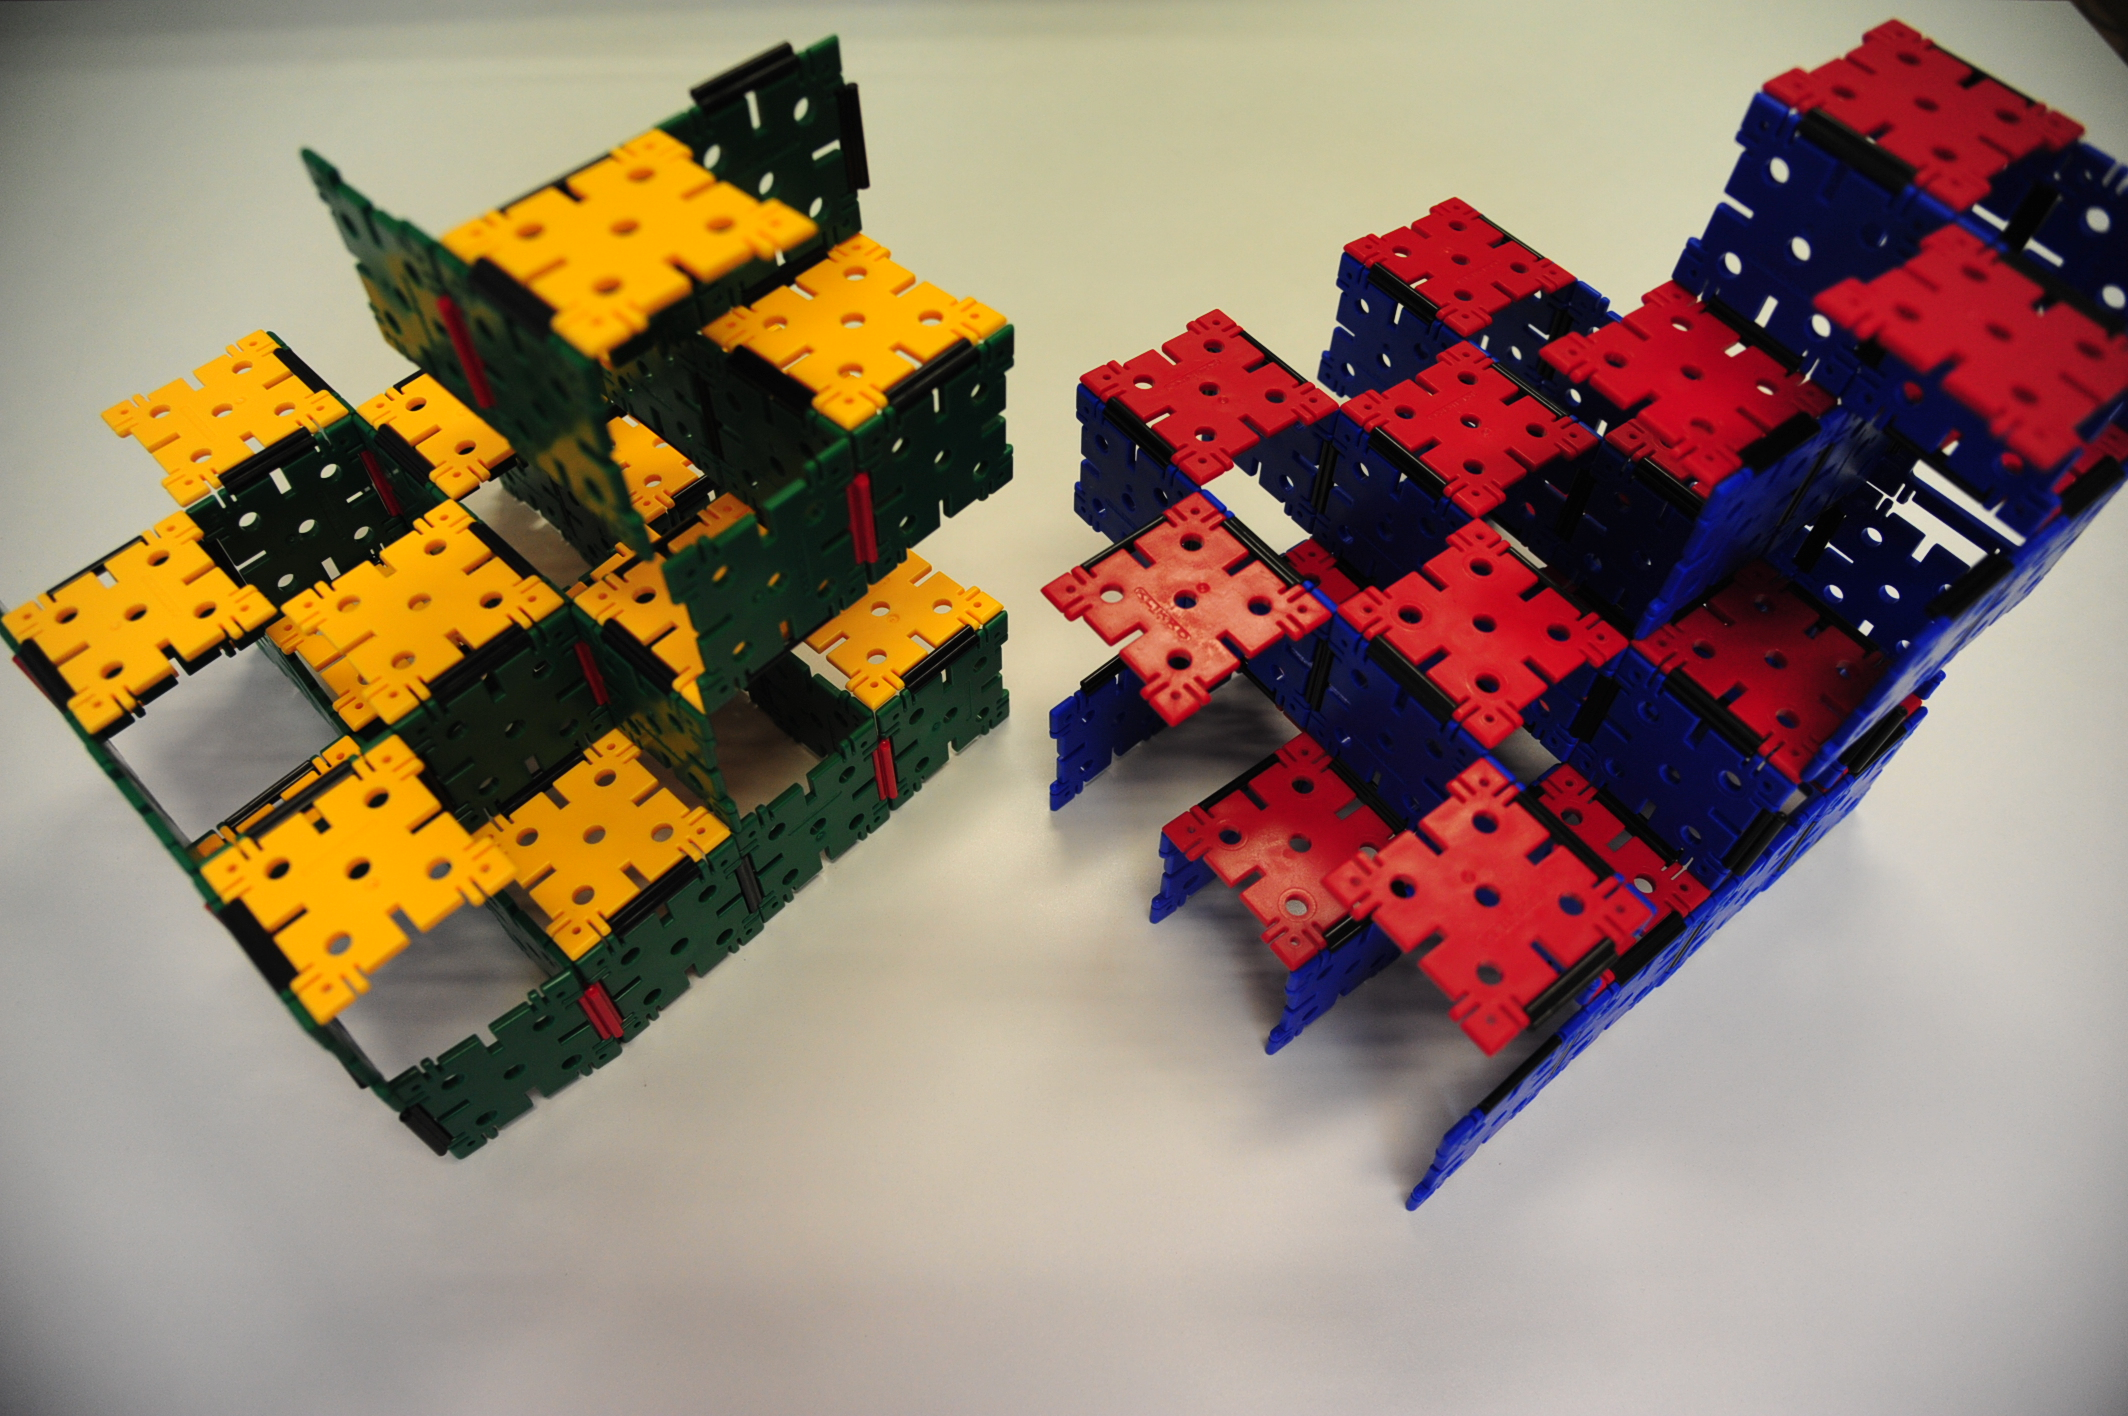
\includegraphics[height=4cm]{toys}
%		\end{center}
%	\end{column}
%	\begin{minipage}[t][0.5\textheight]{0.55\textwidth}
      \tableofcontents[currentsection]
%    \end{minipage}\hfill
%	\end{columns}
\end{frame}
}


% Delete this, if you do not want the table of contents to pop up at
% the beginning of each subsection:

\begin{document}

\begin{frame}
  \titlepage
\end{frame}

\begin{frame}{Collaborators}
  \begin{itemize}
  \item Yunqing Ouyang: Fudan University $\Rightarrow$ Huawei.
  \item Zhi-Da Song: Peking University.
  \item Qing-Rui Wang: Tsinghua University.
  \item Chen Fang: Institute of Physics, Beijing.
  \item Zheng-Cheng Gu: Chinese University of Hong Kong.
    \begin{center}
      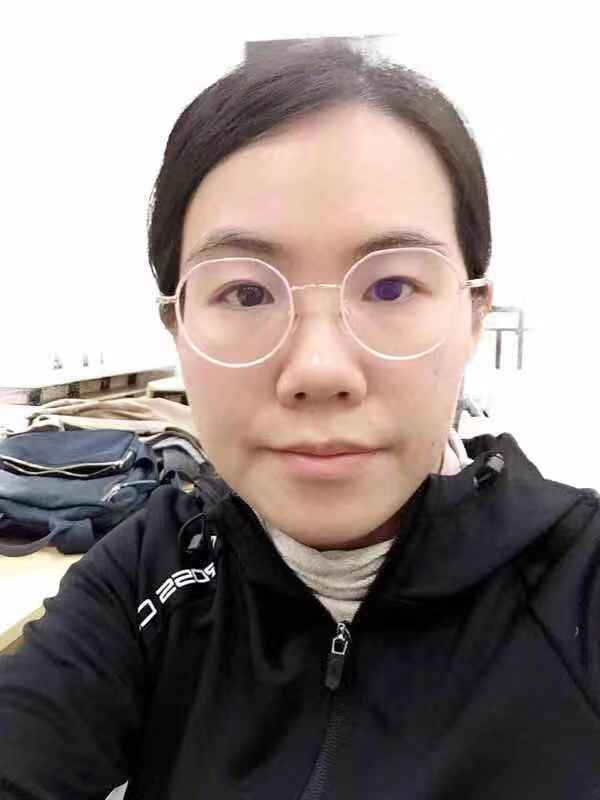
\includegraphics[height=2.5cm]{../people/yunqing}
      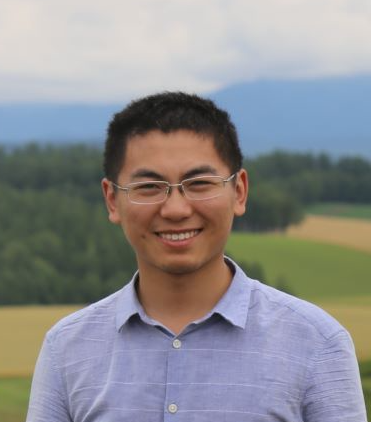
\includegraphics[height=2.5cm]{../people/zhidasong}
      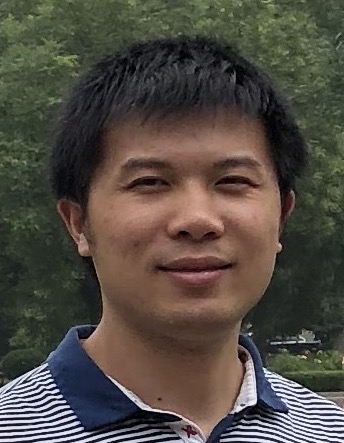
\includegraphics[height=2.5cm]{../people/qingrui}      
      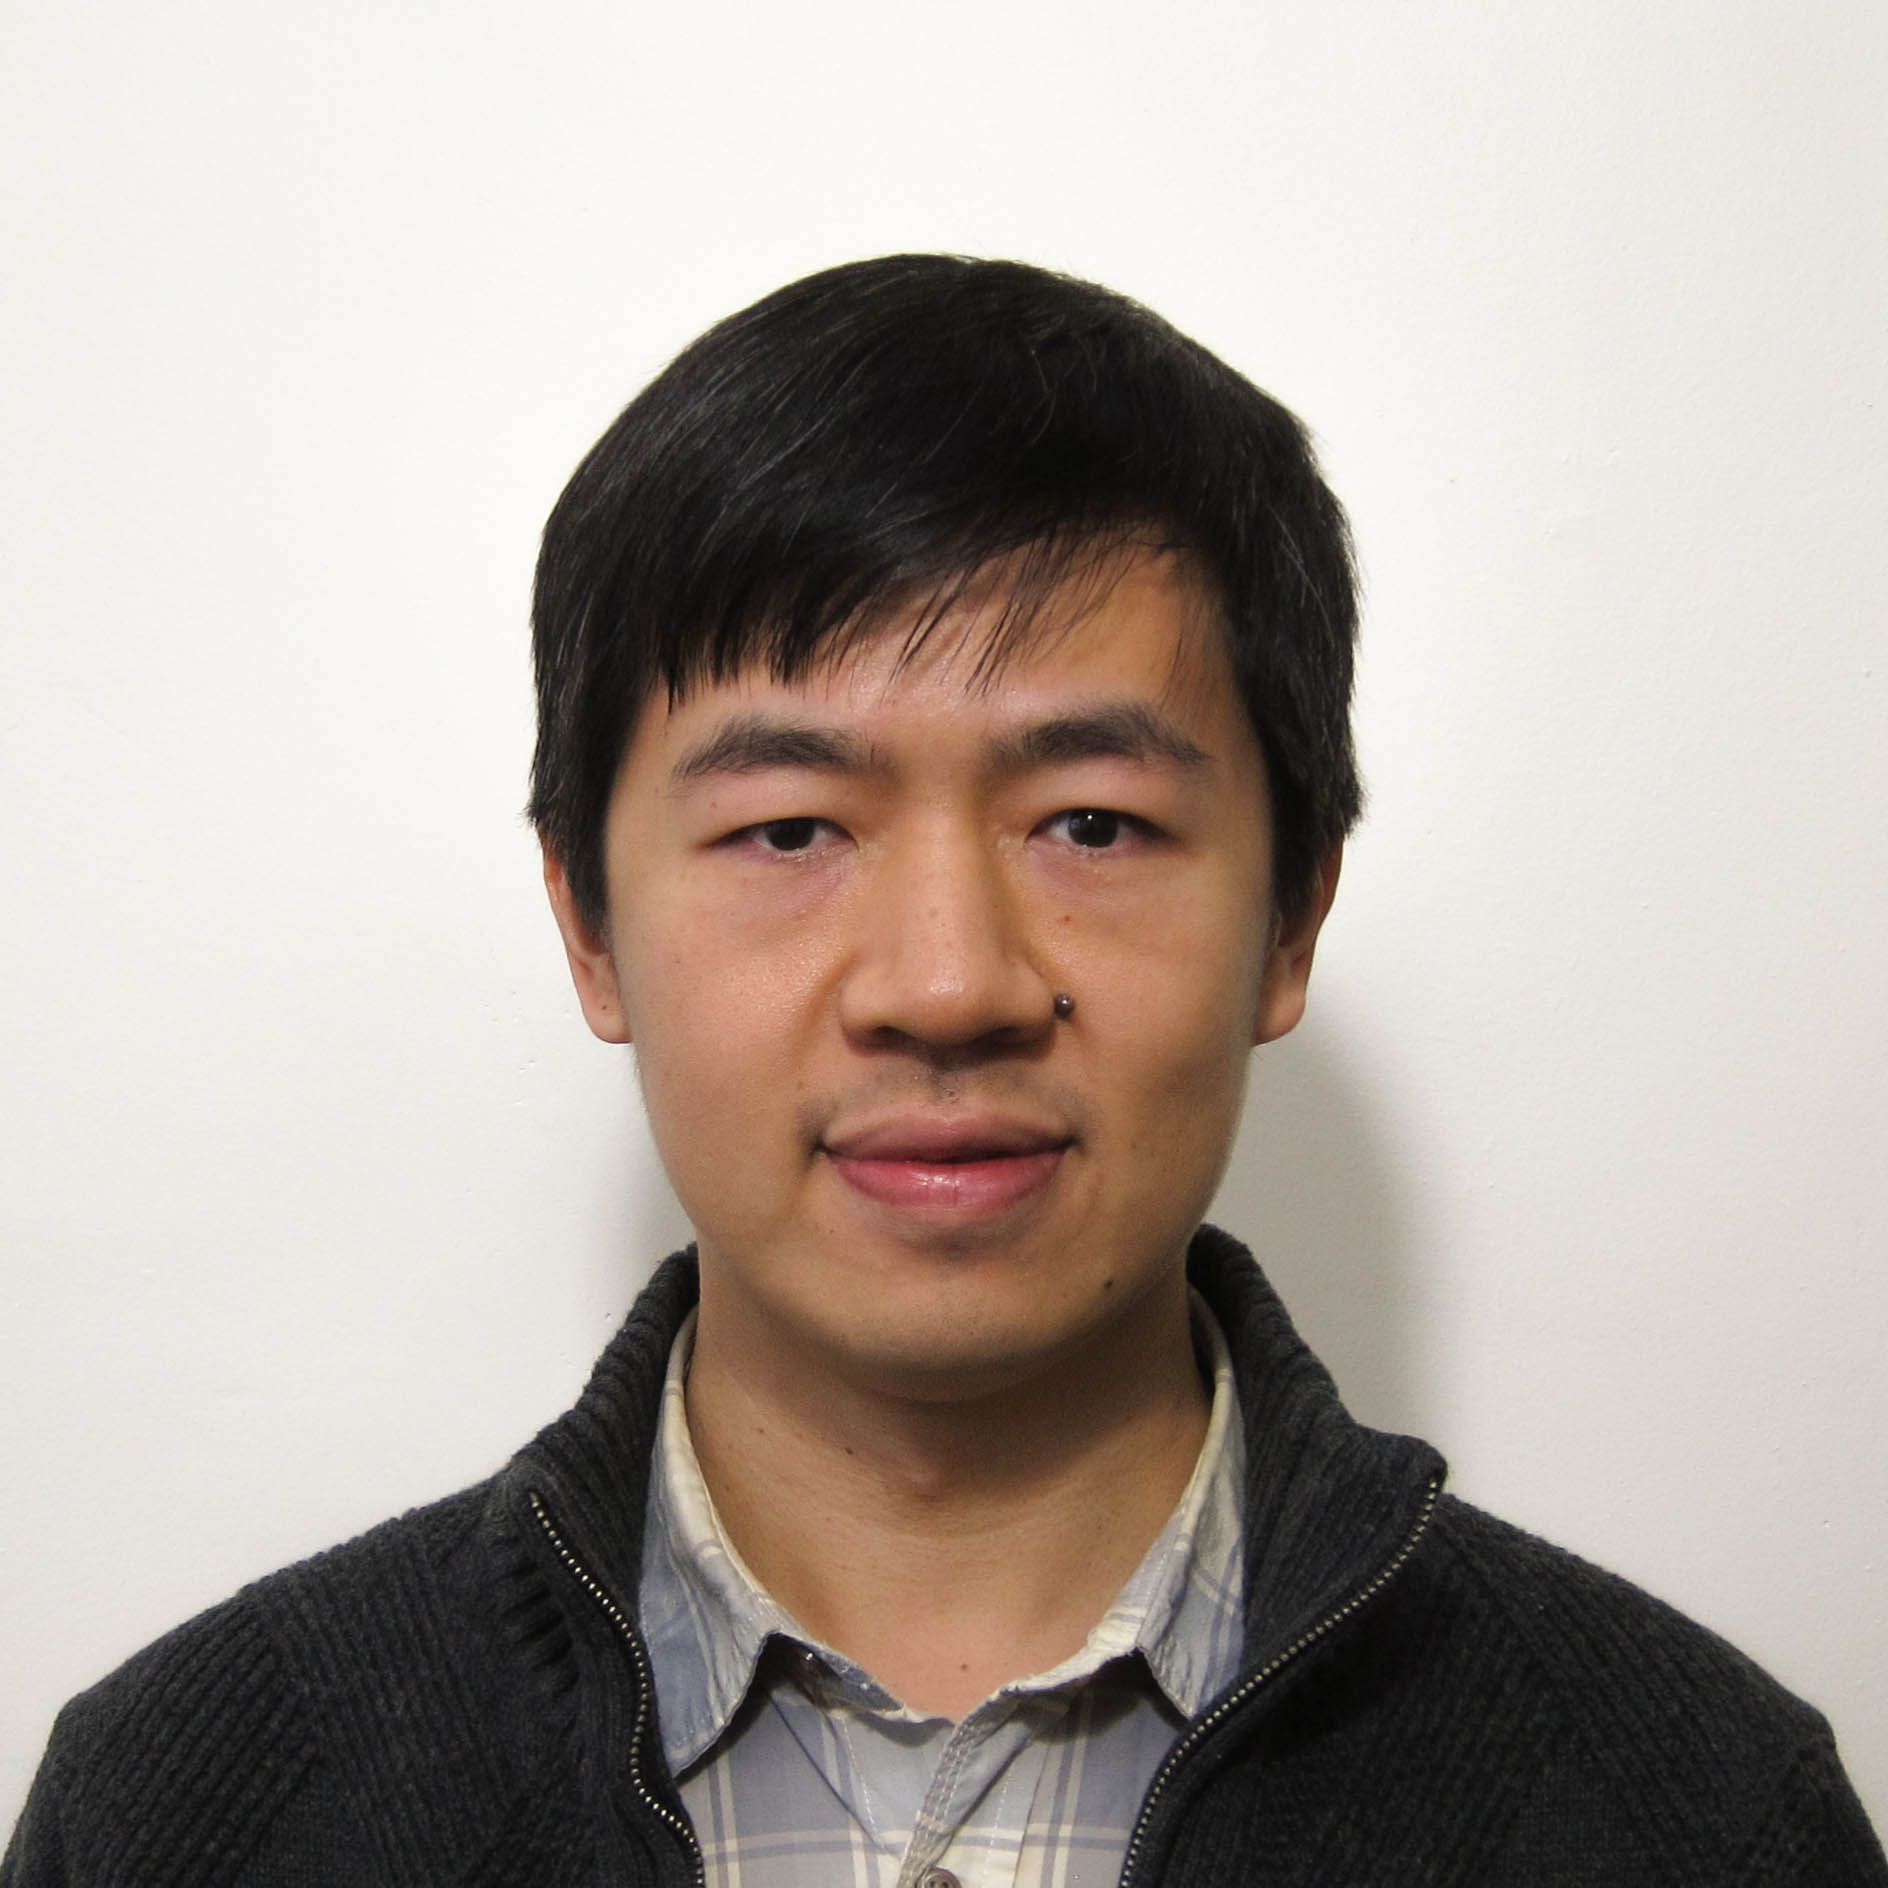
\includegraphics[height=2.5cm]{../people/chenfang}
      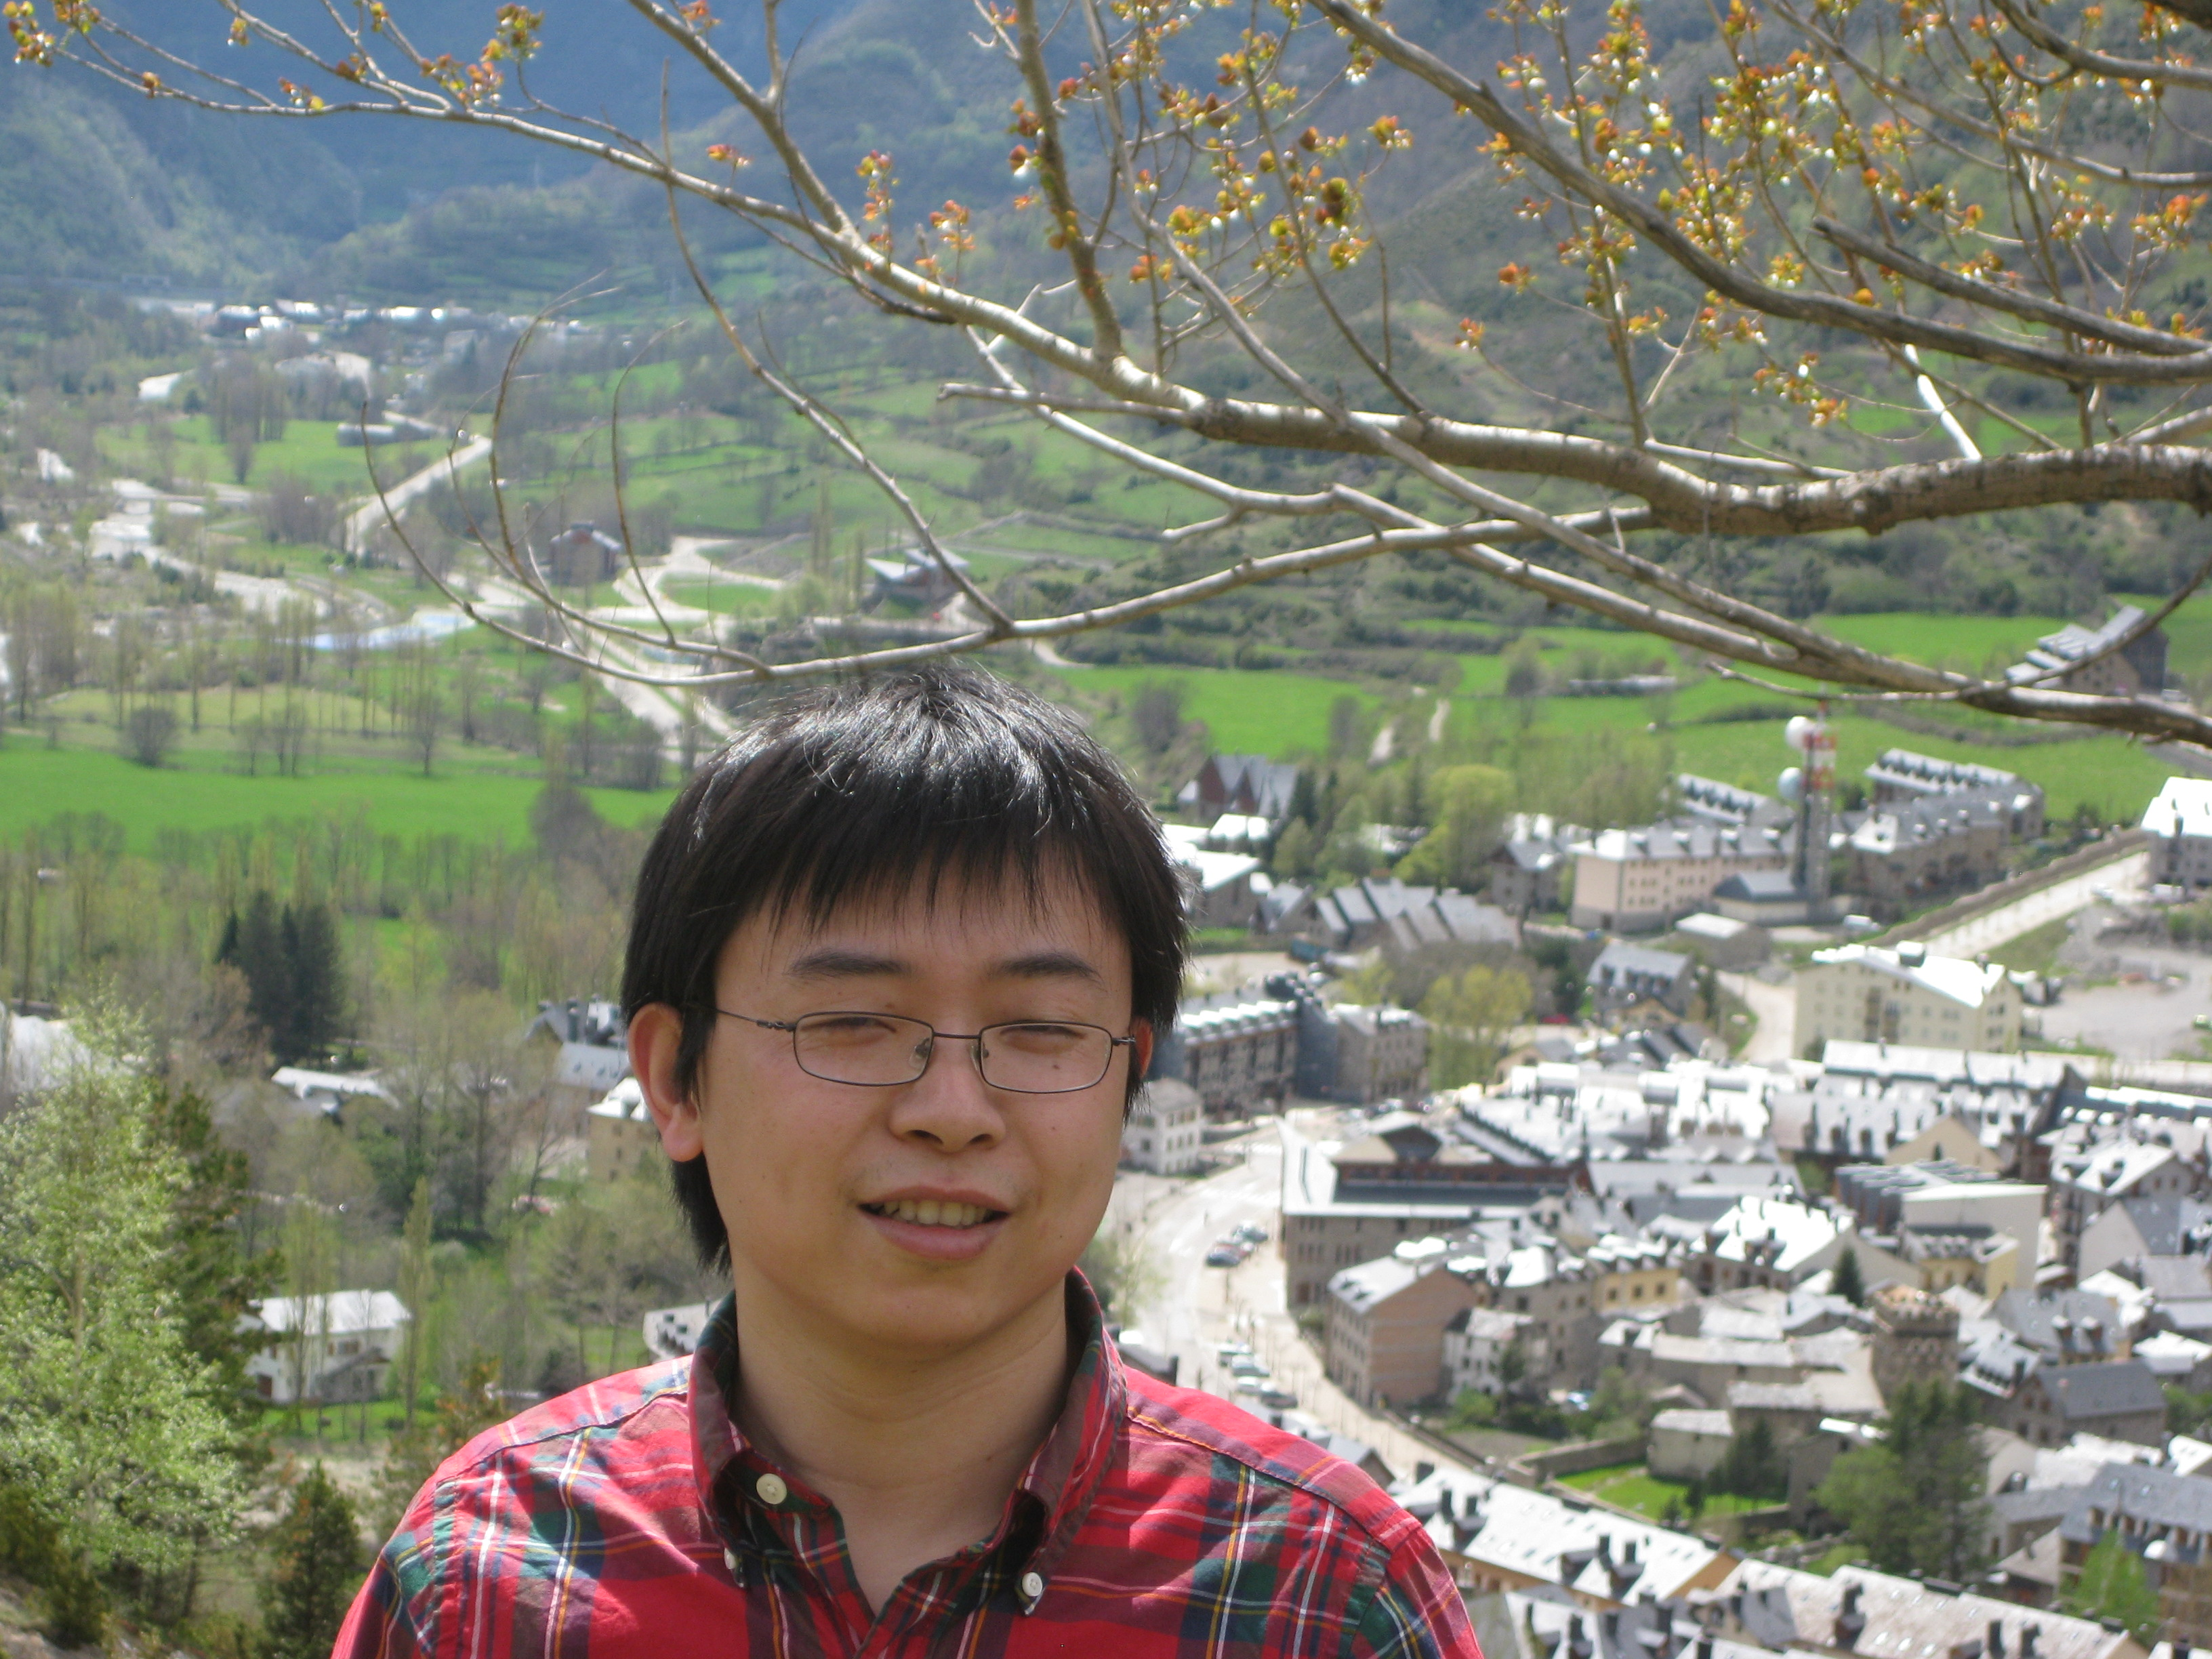
\includegraphics[height=2.5cm]{../people/zhengcheng}
    \end{center}
\end{itemize}
\end{frame}

\begin{frame}{Outline}
%	\begin{columns}
%		\begin{column}[t]{.45\textwidth}
%		\begin{center}
%			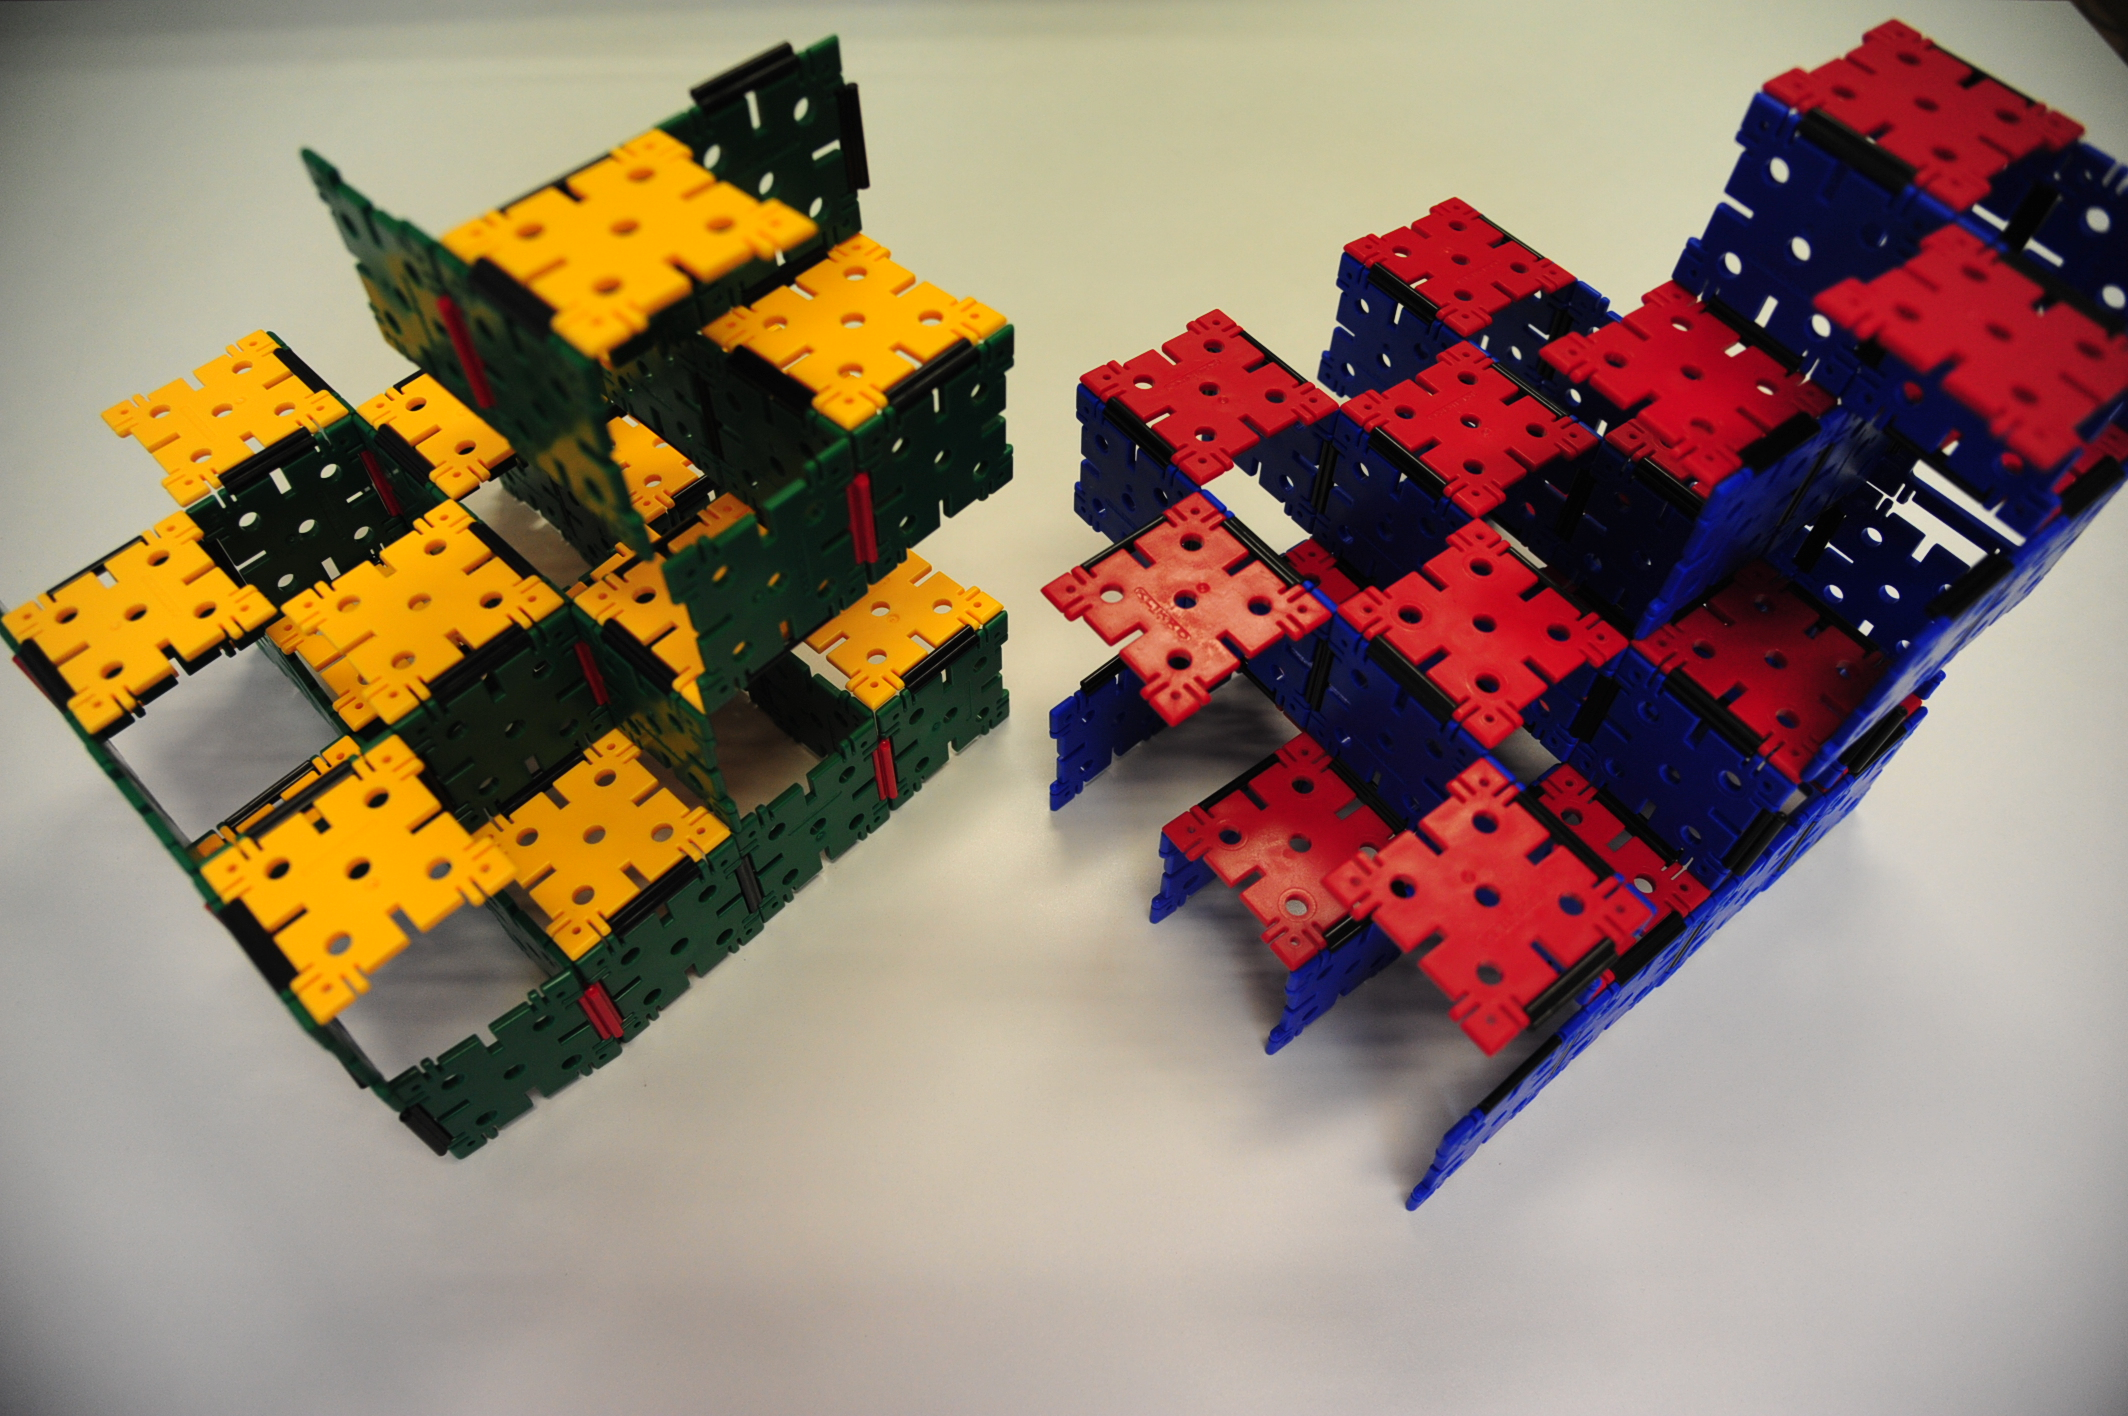
\includegraphics[height=4cm]{toys}
%		\end{center}
%	\end{column}
%	\begin{minipage}[t][0.5\textheight]{0.55\textwidth}
      \tableofcontents
%    \end{minipage}\hfill
%	\end{columns}
\end{frame}


\section{Introduction to SPT States}

\begin{frame}
  \frametitle{Symmetry-Protected Topological (SPT) phases}
  \begin{itemize}
  \item Landau paragidm: phases are classified by symmetry breaking.
    \begin{center}
      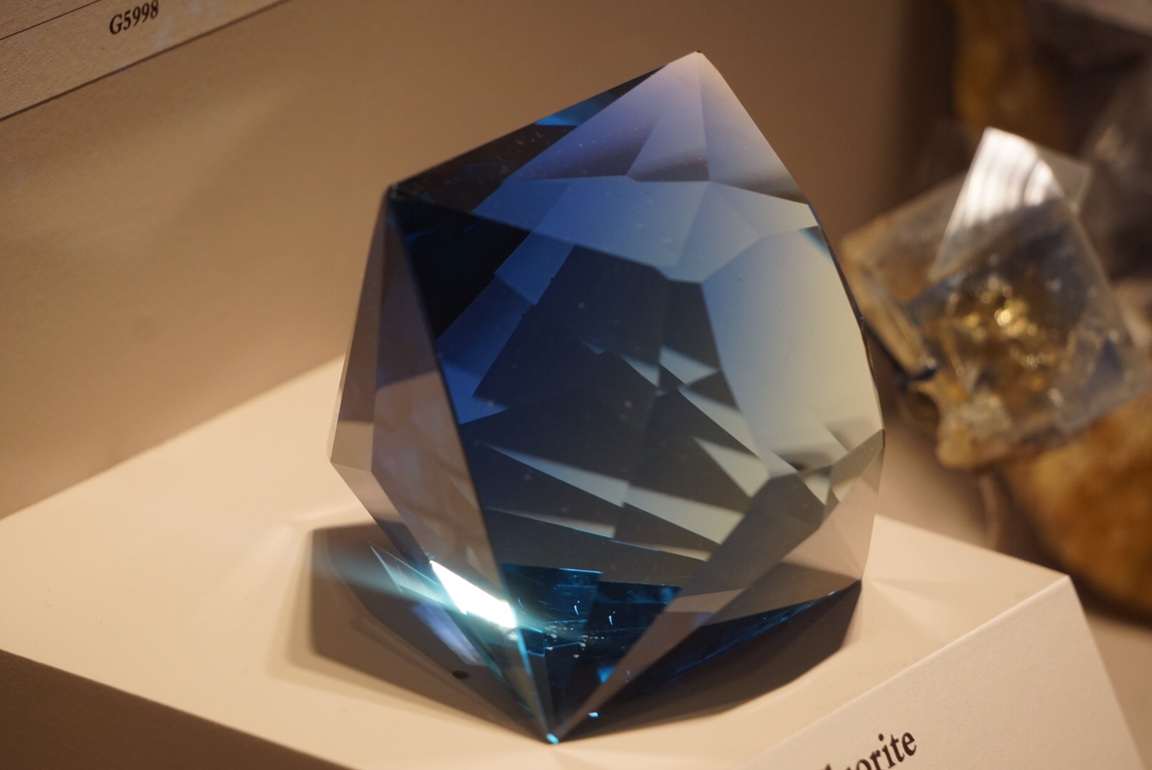
\includegraphics[height=1.5cm]{../resources/crystal}~~
      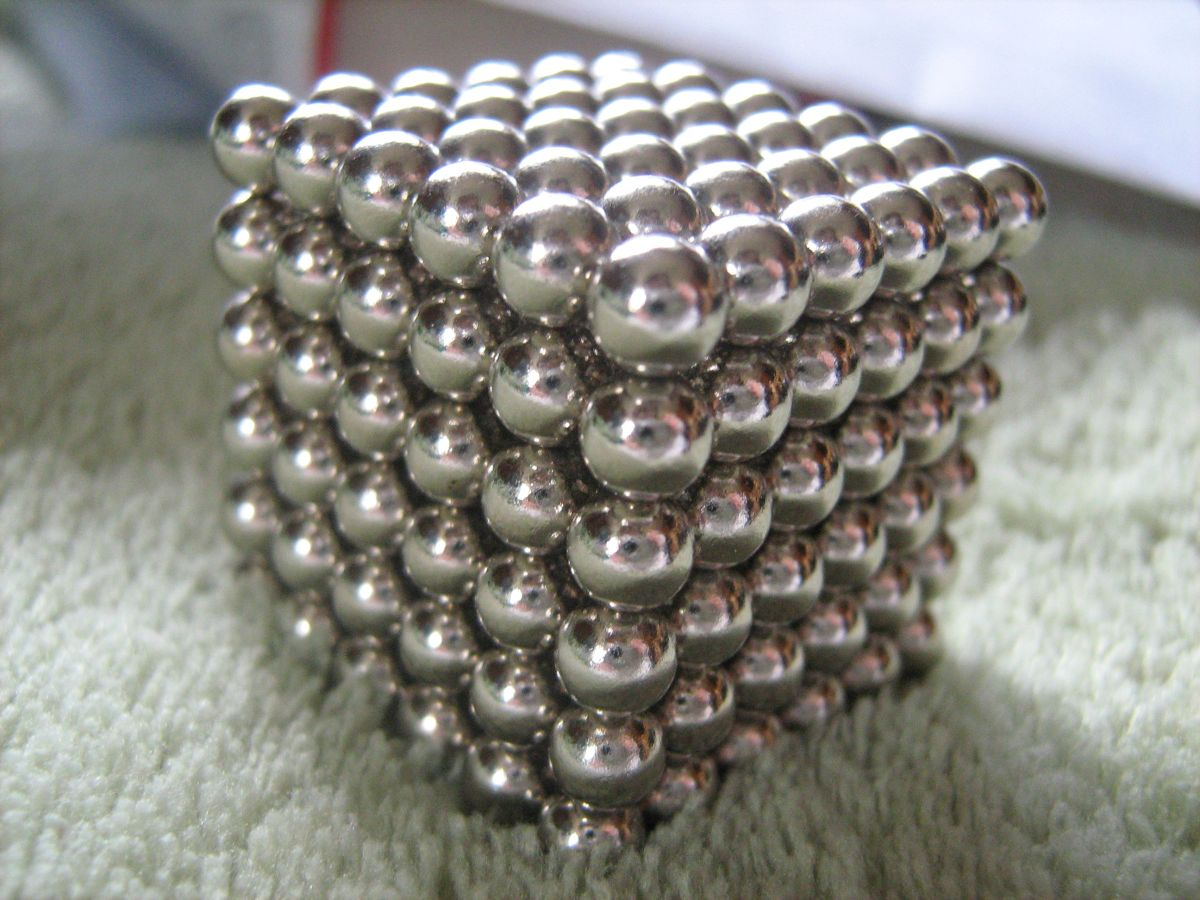
\includegraphics[height=1.5cm]{../resources/magnet}~~
      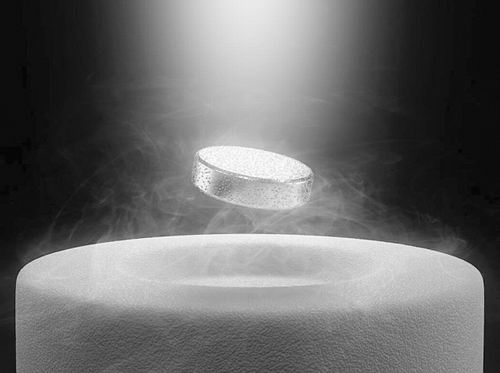
\includegraphics[height=1.5cm]{../resources/sc}
    \end{center}
  \item SPT: gapped topological phases beyond Landau paradiam.
  \item Gapped bulk : cannot be smoothly connected to a trivial state without closing gap or breaking symmetry.
  \item Symmetry-protected gapless surface states.
  \item Example: integer quantum Hall states; topological insulators.
    \begin{center}
      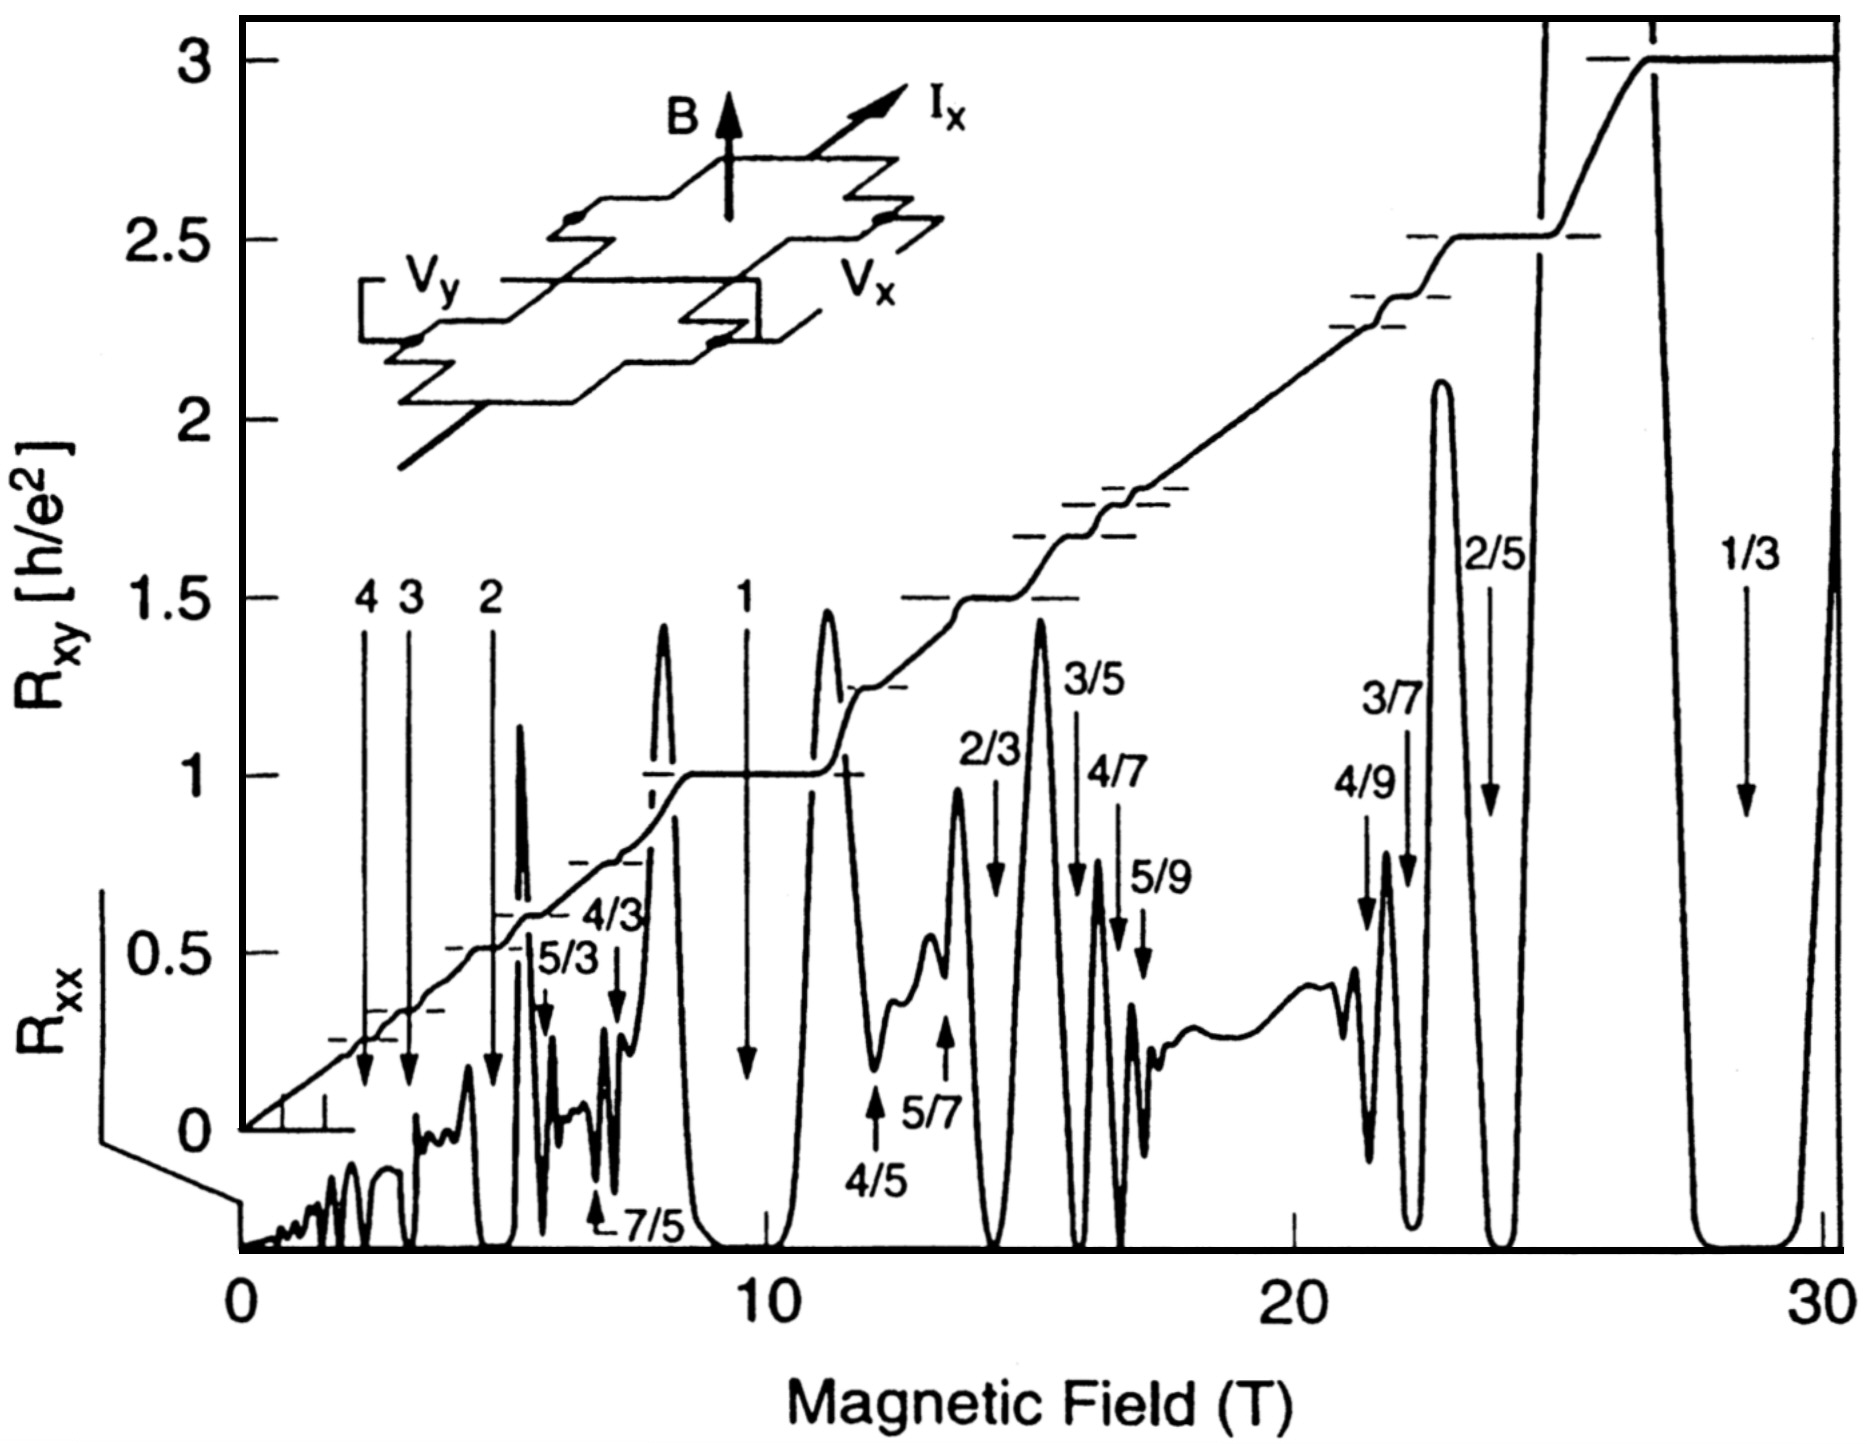
\includegraphics[height=2cm]{../resources/fqhe}~~
      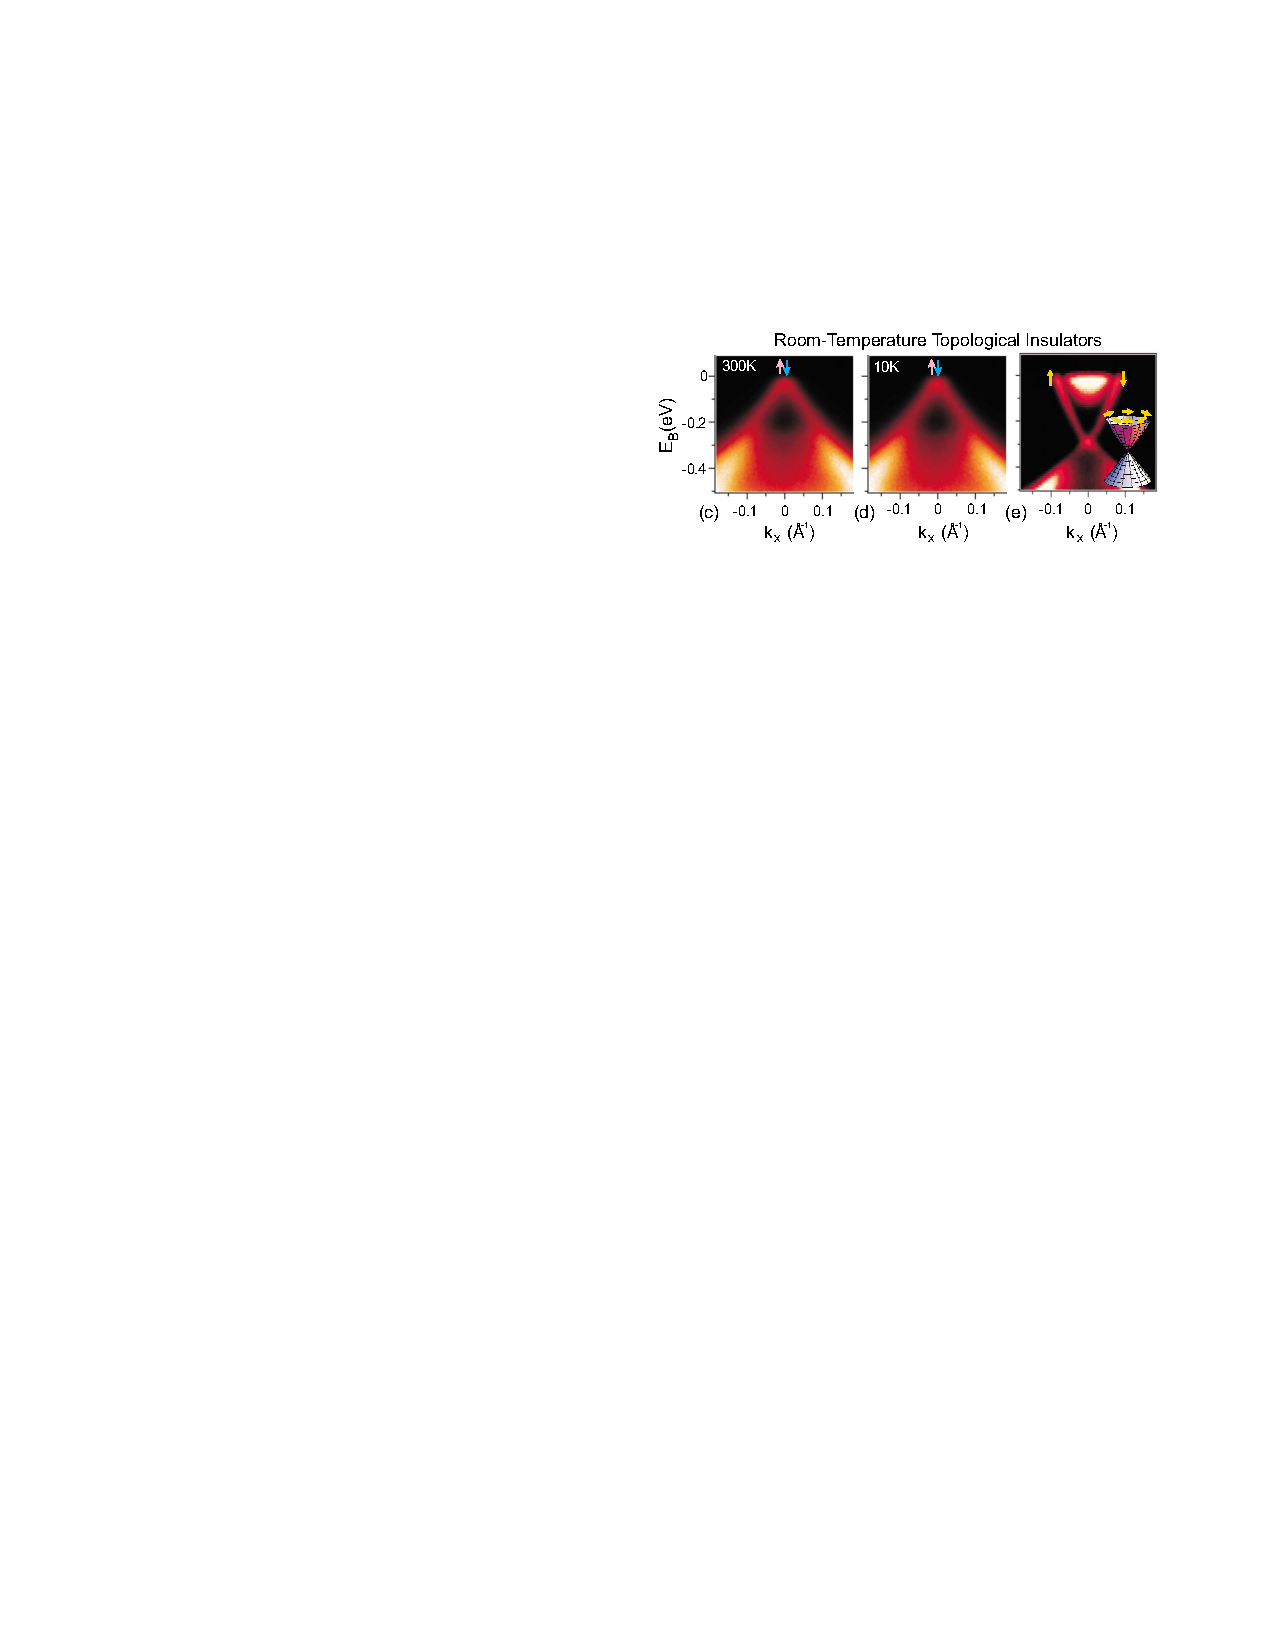
\includegraphics[height=2cm]{ti_surface}
    \end{center}
  \end{itemize}
\end{frame}

\begin{frame}
  \frametitle{Abelian-group classification}
  \begin{itemize}
  \item SPT phases and boundary anomalies are classified by Abelian groups ($\mathbb Z$ or $\mathbb Z_n$).
    \begin{itemize}
    \item Addition: stacking of phases/gapless boundaries.
    \item 0: The trivial phase/gapped boundary.
    \end{itemize}
  \item Classification: determined by symmetry group $G$ and dimension $d$.
  \item 2D Chern-insulators (Integer Quantum Hall):
    \begin{center}
      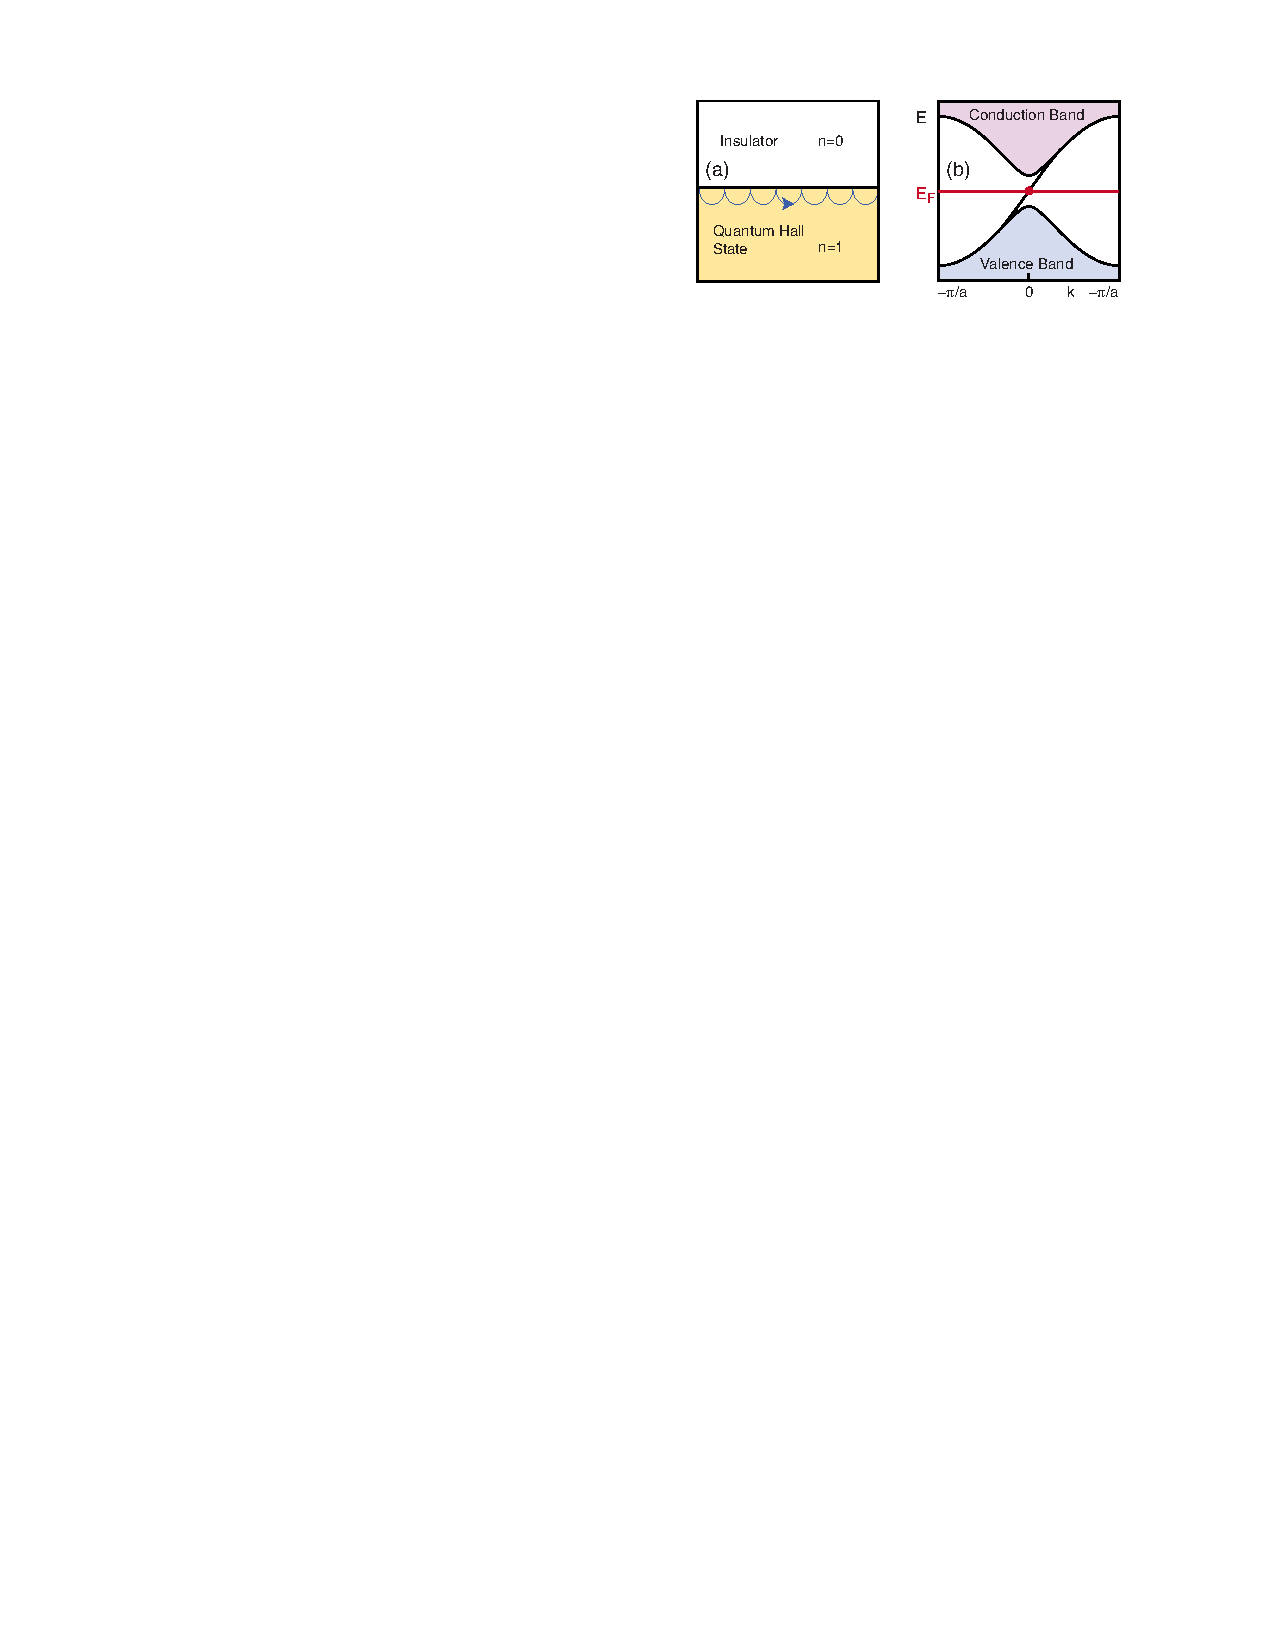
\includegraphics[width=8cm]{qhe_edge}
    \end{center}
    Classified by $\mathbb Z$: $[n]+[m]=[n+m]$; $[n]+[-n] = 0$.
  \end{itemize}
\end{frame}

\begin{frame}
	\frametitle{Abelian-group classification}
	\begin{itemize}
		\item 3D Topological Insulators:
		\begin{center}
			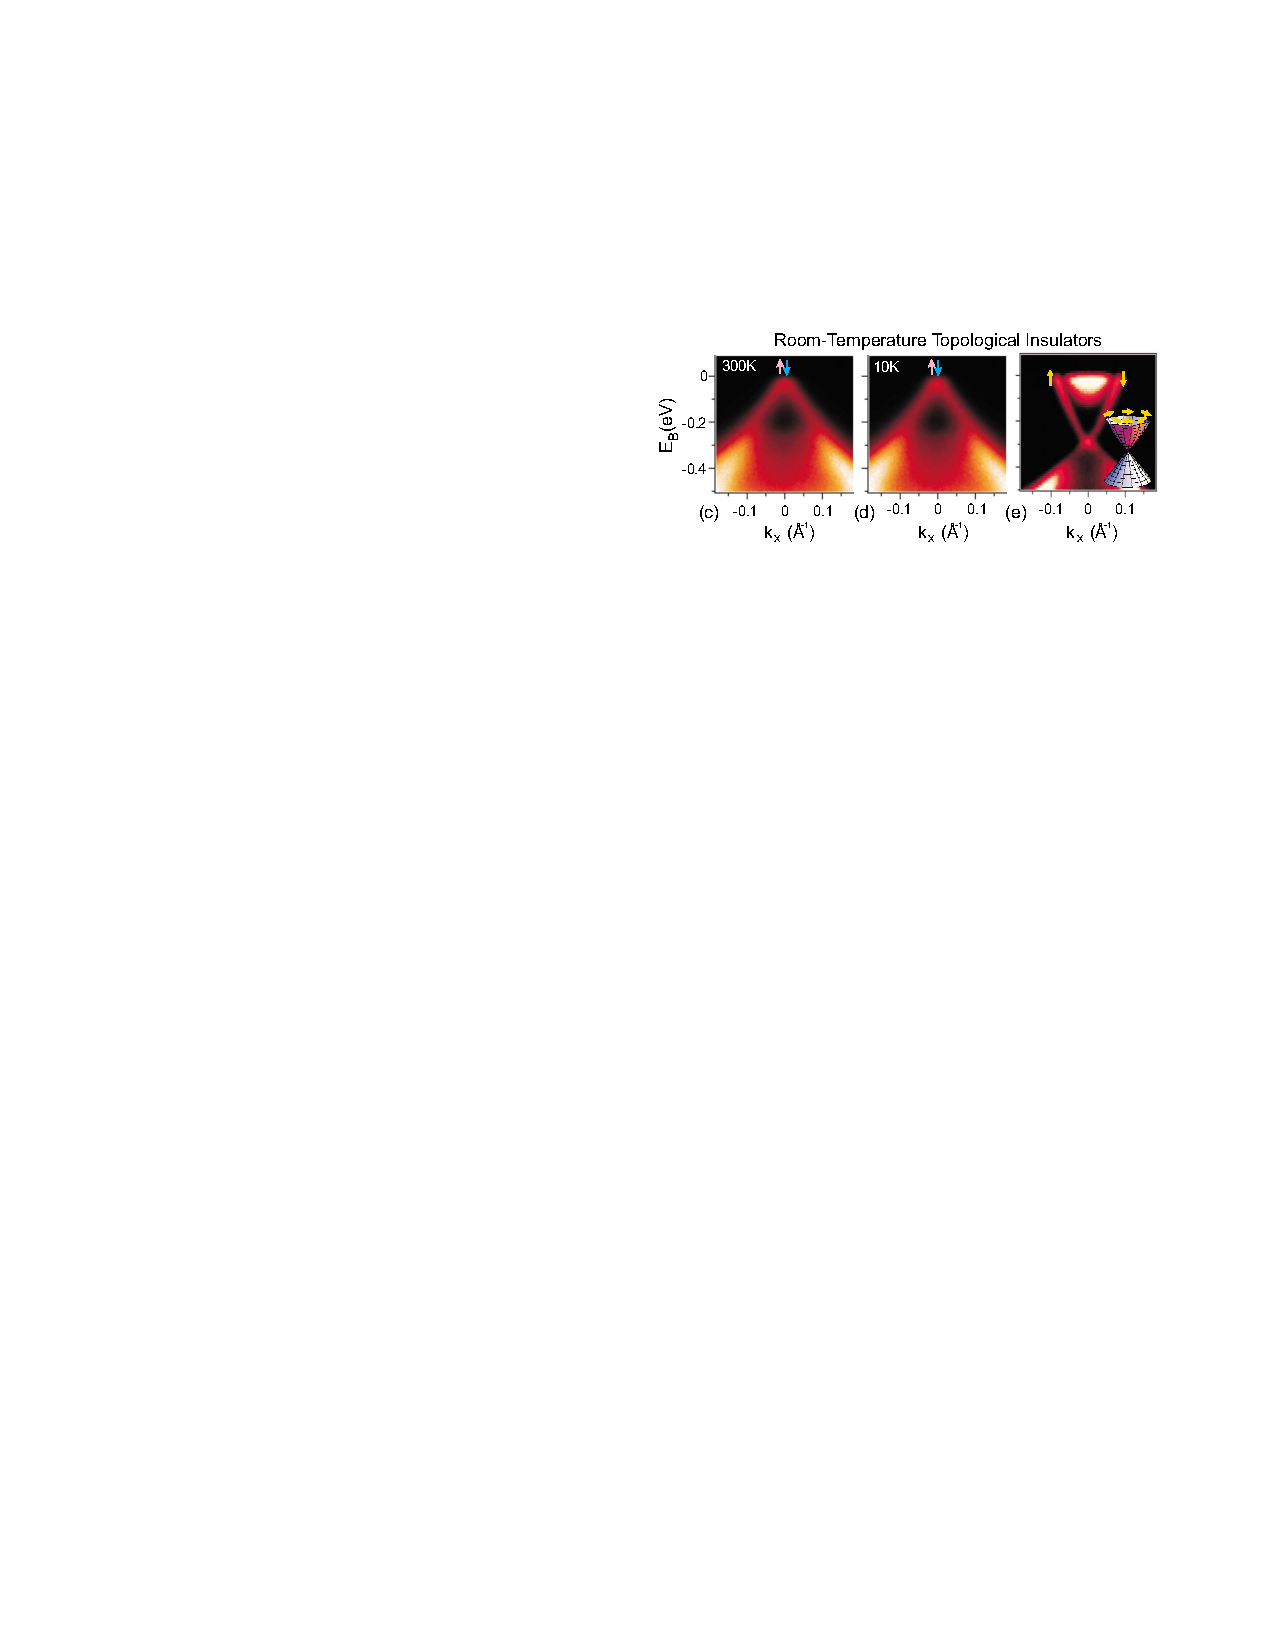
\includegraphics[width=8cm]{ti_surface}
		\end{center}
		Classified by $\mathbb Z_2$: $[1]+[1] = 0$.
		\item 1D Haldane chain:
		\begin{center}
			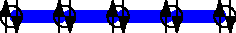
\includegraphics[width=6cm]{../dimer/weak3d_aklt_blue}
		\end{center}
		Classified by $\mathbb Z_2$: $[1]+[1] = 0$.
	\end{itemize}
\end{frame}

\begin{frame}{SPT 101}
  What do we need to know about classification of SPT phases?
  \begin{itemize}
  \item Forms an Abelian group.
  \item Determined by a symmetry group $G$ and spatial dimension $d$: $\Phi^d(G)$.
    %\begin{itemize}
    %\item Forgetting symmetries: $H$ is a subgroup of $G$: $\Phi^d(G)\rightarrow\Phi^d(H).$
    %\item Group isomorphism: $G\simeq G'$: $\Phi^d(G)\simeq \Phi^d(G')$.
    %\item Calculation rules can be precisely formulated.
    %\end{itemize}
  \item A (generalized) cohomology theory $\Phi^d(G)=\mathcal H^{d+1}(G)$.
  \end{itemize}
  \begin{enumerate}
    \item Free-fermion states: topological insulators, topological superconductors; K-theory.
    \emph{A. Kiraev, AIP Conf. Proc. 1134, 22 (2009).}
    \item Bosonic SPTs: Haldane chain, CZX/Levin-Gu state; group-cohomology theory.
    \emph{Xie Chen, Zheng-Cheng Gu, Zheng-Xin Liu and Xiao-Gang Wen, Science 2012.}
        \item Interacting fermionic SPTs: a ``generalized'' cohomology theory.
  \end{enumerate}
  \end{frame}


\begin{frame}
\frametitle{Topological Crystaline States = Space-group SPT}
\begin{itemize}
\item Two approaches:
  \begin{enumerate}
  \item Thorngren and Else (2018): the crystalline equivalence principle
    \[SG\simeq G;\quad \Phi^d(SG)\simeq\Phi^d(G).\]
  \item Dimensional reduction: Liang Fu, Michael Hermele et al.\\
    \emph{Examples: mirror SPT, weak SPT (translation symmetry).}
    %\emph{Patch construction: Zhida Song, Shengjie Huang, YQ, Chen Fang and Michael Hermele, Sci. Adv. 5, eaax2007 (2019).}
  \end{enumerate}
\item A more general construction for bosonic/fermionic SPTs w/ all possible $G$?
\end{itemize}
\begin{center}
\begin{tikzpicture}[scale=.9]
\fill [blue!20] (0,0)--(1,1)--(1,3)--(0,2)--(0,0);
\draw (0,0)--(0,2)--(1,3);
\draw (-1.5,0)--(1.5,0)--(1.5,2)--(-1.5,2)--(-1.5,0);
\draw (1.5,0)--(2.5,1)--(2.5,3)--(1.5,2);
\draw (2.5,3)--(-.5,3)--(-1.5,2);
\end{tikzpicture}
\hspace{2em}
\begin{tikzpicture}[scale=.9]
\fill [blue!40,opacity=.5] (0,0)--(1,1)--(1,3)--(0,2)--(0,0);
\draw (0,0)--(0,2)--(1,3);
\fill [blue!40,opacity=.5] (.5,0)--(1.5,1)--(1.5,3)--(0.5,2)--(0.5,0);
\draw (.5,0)--(.5,2)--(1.5,3);
\fill [blue!40,opacity=.5] (1,0)--(2,1)--(2,3)--(1,2)--(1,0);
\draw (1,0)--(1,2)--(2,3);
\fill [blue!40,opacity=.5] (-.5,0)--(.5,1)--(.5,3)--(-0.5,2)--(-0.5,0);
\draw (-.5,0)--(-.5,2)--(.5,3);
\fill [blue!40,opacity=.5] (-1,0)--(0,1)--(0,3)--(-1,2)--(-1,0);
\draw (-1,0)--(-1,2)--(0,3);
\draw (-1.5,0)--(1.5,0)--(1.5,2)--(-1.5,2)--(-1.5,0);
\draw (1.5,0)--(2.5,1)--(2.5,3)--(1.5,2);
\draw (2.5,3)--(-.5,3)--(-1.5,2);
\end{tikzpicture}
\end{center}
\end{frame}

\begin{frame}{Why Topological Crystaline States?}
  \begin{itemize}
    \item Crystalline symmetries are present in all solid-state materials.
    \item High-order boundary states: TCSs (excluding the Atomic Insulators) are a.k.a. High-Order Topological States.
    May be useful for storing quantum information.
  \end{itemize}
  \begin{center}
    \begin{tikzpicture} [scale=2]
      \fill [blue!50] (0,0)--(1,0)--(1.5,.5)--(1.5,1.5)--(0.5,1.5)--(0,1)--(0,0);
      \draw [thick,red] (0,0)--(1,0)--(1,1)--(0,1)--(0,0);
      \draw [thick,red] (1,0)--(1.5,.5)--(1.5,1.5)--(1,1);
      \draw [thick,red] (1.5,1.5)--(0.5,1.5)--(0,1);
      \draw [thick,red] (0,0)--(.5,.5)--(.5,1.5);
      \draw [thick,red](.5,.5)--(1.5,.5);
      \fill [red] (0,0) circle (2pt);
      \fill [red] (1,0) circle (2pt);
      \fill [red] (0,1) circle (2pt);
      \fill [red] (1,1) circle (2pt);
      \fill [red] (0.5,0.5) circle (2pt);
      \fill [red] (1.5,0.5) circle (2pt);
      \fill [red] (0.5,1.5) circle (2pt);
      \fill [red] (1.5,1.5) circle (2pt);
    \end{tikzpicture}      
  \end{center}
\end{frame}

\section{Approach I: use crystalline equivalence principle}

\begin{frame}
  \frametitle{Crystalline equivalence principle}
  \begin{itemize}
  \item SPT classification remains the same, if:
    \begin{enumerate}
    \item Crystalline symmetry group $\Rightarrow$ onsite symmetry group.\\
      \emph{Example: $C_2$-SPT = $\mathbb Z_2$-SPT.}
    \item Symmetries reversing space orientation $\Rightarrow$ antiunitary symmetries.\\
      \emph{Example: mirror reflection, glide phane, ...}
    \item For fermions: spinless/spin-$\frac12$ $\Rightarrow$ spin-$\frac12$/spinless.\\
      \emph{Example: $C_2^2=\pm1 \Rightarrow g^2=\mp1$.}
    \end{enumerate}
  \item We can compute crystalline-SPT as onsite-SPTs.
  \item Large symmetry groups (space groups are infinite): need an efficient algorithm.
  \end{itemize}
  \begin{center}
    \begin{tikzpicture}
      \draw (-6, -1.5)--(-6, 1.5)--(-3, 1.5)--(-3, -1.5)--(-6, -1.5);
    \draw [->] (-5, .3)--(-5, .7);
    \draw [->] (-4, .3)--(-4, .7);
    \draw [->] (-5, -.3)--(-5, -.7);
    \draw [->] (-4, -.7)--(-4, -.3);
    \node at (-2.25, 0) {=};

    \draw (-1.5, -1.5)--(-1.5, 1.5)--(1.5, 1.5)--(1.5, -1.5)--(-1.5, -1.5);
    \draw [->] (.7, 0) arc (0:180:0.7);
    \filldraw (0, 0) circle (1pt) node [right] {$C_2$};
\end{tikzpicture}    
  \end{center}
\end{frame}

%\subsection{Bosonic SPTs}

% \begin{frame}[fragile]{bSPTs: Group cohomology (and beyond)}
%   \begin{itemize}
%     \item Classification: group cohomology $H^{d+1}[G, \uone_{PT}]$.
%     \item Beyond group cohomology: Xiao-Gang Wen,	Phys. Rev. B 91, 205101 (2015).\\
%     \emph{\small Similar to fSPT's domain-wall decoration, but w/ 2d E8 state. More on this later.}
%     \item How to compute: use HAP package in GAP (\url{www.gap-system.org})
%     \begin{lstlisting}[basicstyle=\footnotesize]
%       gap> SG := SpaceGroupBBNWZ(3, 100);;
%       gap> iso := IsomorphismPcpGroup(SG);;
%       gap> SG1 := Image(iso);;
%       gap> gens := GeneratorsOfGroup(SG);;
%       gap> gs1 := List(gens, x->Image(iso, x));;
%       gap> signs := List(gens, x->[[DeterminantMat(x)]]);;
%       gap> f:= GroupHomomorphismByImagesNC(SG1,GL(1,Integers),gs1,signs);;
%       gap> R := ResolutionAlmostCrystalGroup(SG1, 6);;
%       gap> cocc := HomToIntegralModule(R, f);;
%       gap> Cohomology(cocc, 4);
%       [ 2, 2, 2, 4 ]
%     \end{lstlisting}
%     This shows $H^4[SG, \uone_{PT}]=3\mathbb Z_2\oplus\mathbb Z_4$.
%   \end{itemize}
% \end{frame}

%\subsection{Interacting fermionic SPTs}

\begin{frame}
  \frametitle{fSPT w/ onsite symmetry: domain-wall decoration}
  \begin{itemize}
    \item Picture: domain-wall decoration.
    \item How to get a symmetric state?
    \begin{enumerate}
      \item Start from a symmetry-breaking state.
      \item Consider domain configurations.
      \item \alert{Decorate domain walls with different topological states.}
      \item Proliferate domains: construct a coherent superposition of different domain configurations.
    \end{enumerate}
    \item What can we decorate?\\
    invertible Topological Orders: complex fermion; Kitaev chain; (p+ip) SC; ...
  \end{itemize}
  \begin{columns}
    \column{.6\textwidth}
  \begin{center}
    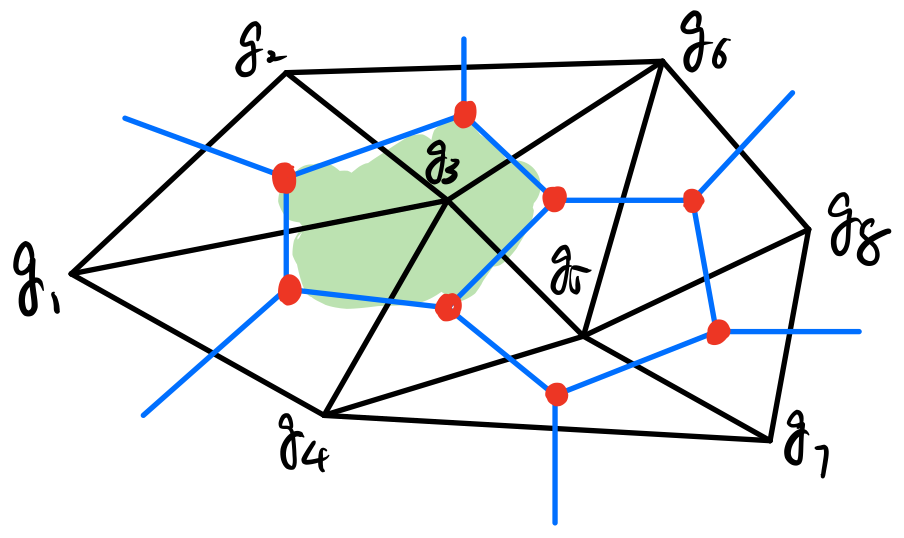
\includegraphics[height=2.5cm]{../chainmap/decoration.png}
  \end{center}
  \column{.4\textwidth}
  \[|\Psi\rangle=\sum_{\{g_i\}}\Bigg|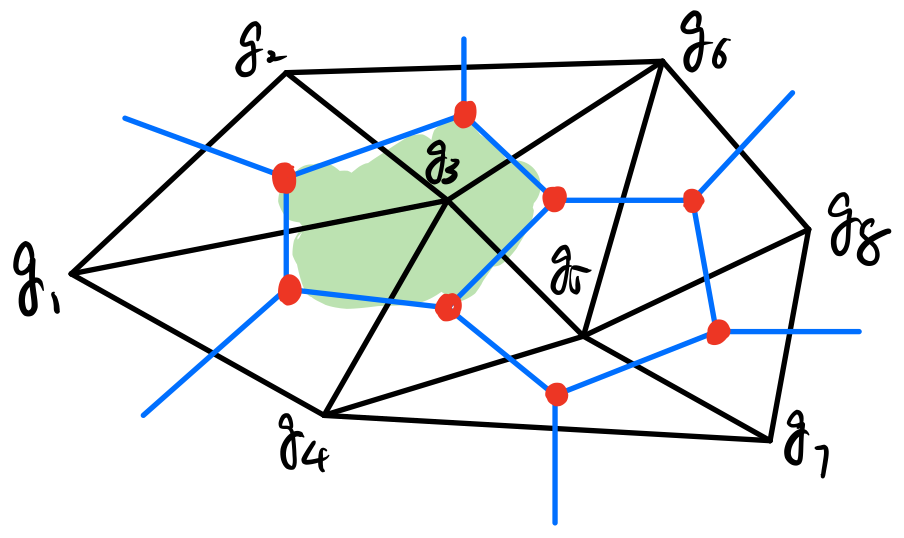
\includegraphics[height=1cm]{../chainmap/decoration.png}\Bigg>\]
  \end{columns}
\end{frame}

\begin{frame}
  \frametitle{fSPT: algebraic description}
  \begin{itemize}
    \item SPT classification: generalized cohomology theory of symmetry group $G$.
    \item Atiyah–Hirzebruch Spectral Sequence: SPT of interacting fermions are described by combinations of cochains:
      \[E^{pq}_2=H^p(G, \text{iTO}^q)\Rightarrow
      \mathcal H^{p+q}(G).\]
    \item Decorating domain walls and sum over all domain configurations.
      \[(2+1)d: n_1(g_1); n_2(g_1, g_2); \nu_3(g_1,g_2,g_3).\]
    \item $n_1$ and $n_2$: decoration of invertible topological states.
    \item $\nu_3$: relative phase b/w different configurations.
  \end{itemize}
  \begin{center}
    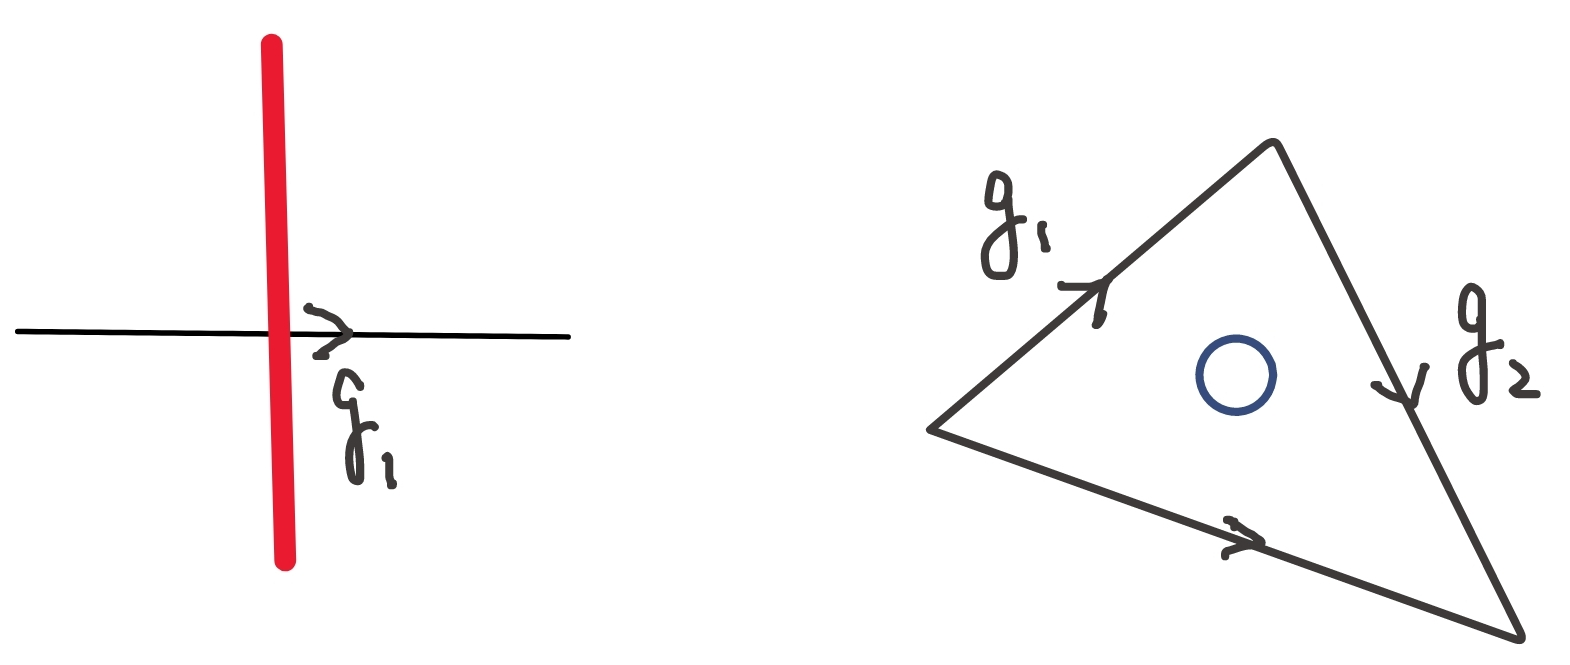
\includegraphics[height=2.5cm]{fspt_decor.jpg}
    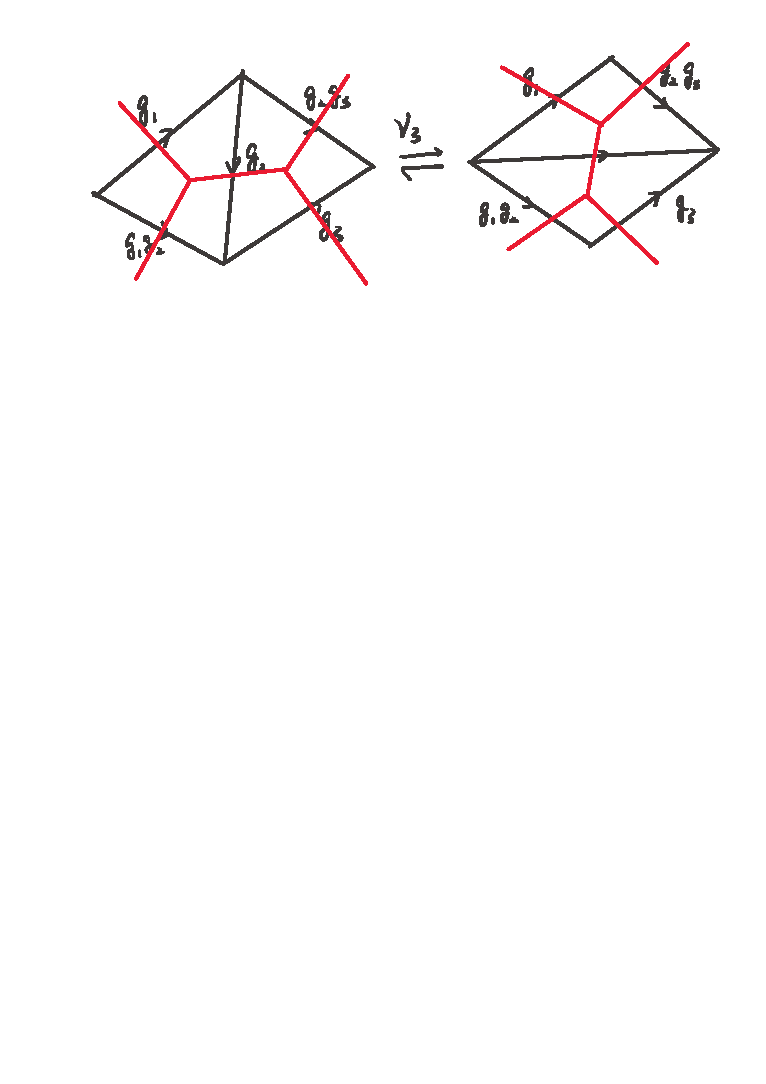
\includegraphics[height=2.5cm]{fmove2.pdf}
  \end{center}
\end{frame}

\begin{frame}{Obstruction functions}
  \begin{itemize}
    \item Example: constraints on $\nu_3$, frustration-free $\Rightarrow$ ``pentagon equation''.
    \begin{center}
      %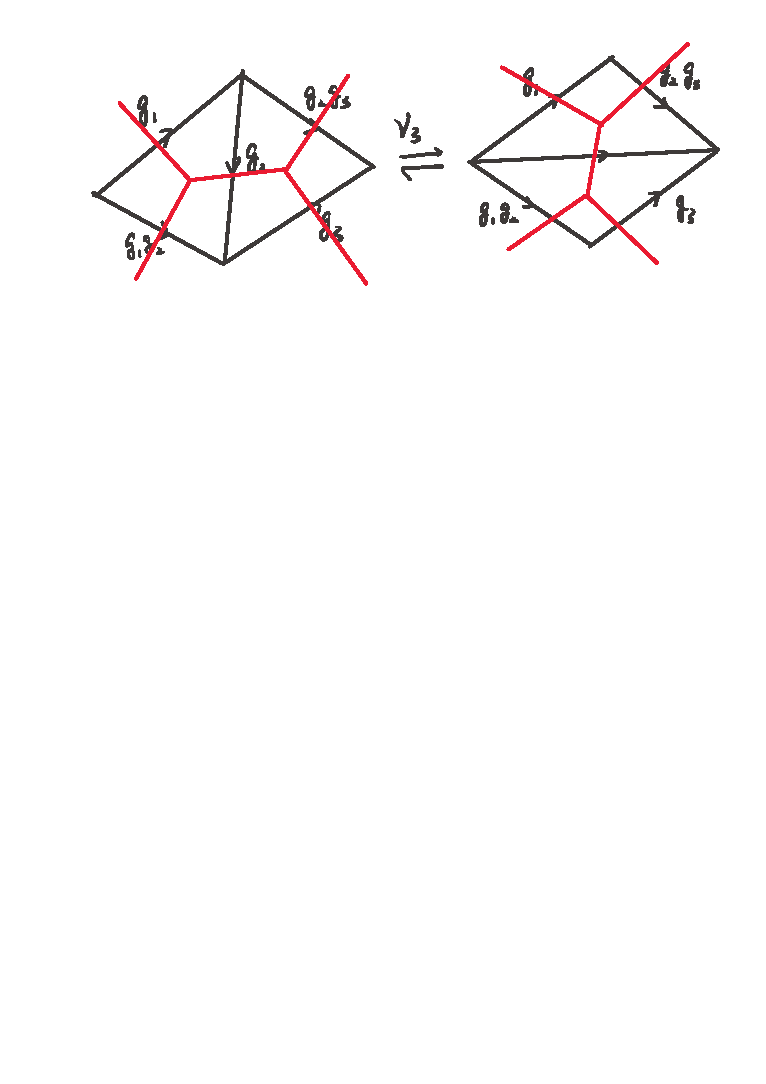
\includegraphics[height=2cm]{fmove2.pdf}\\
      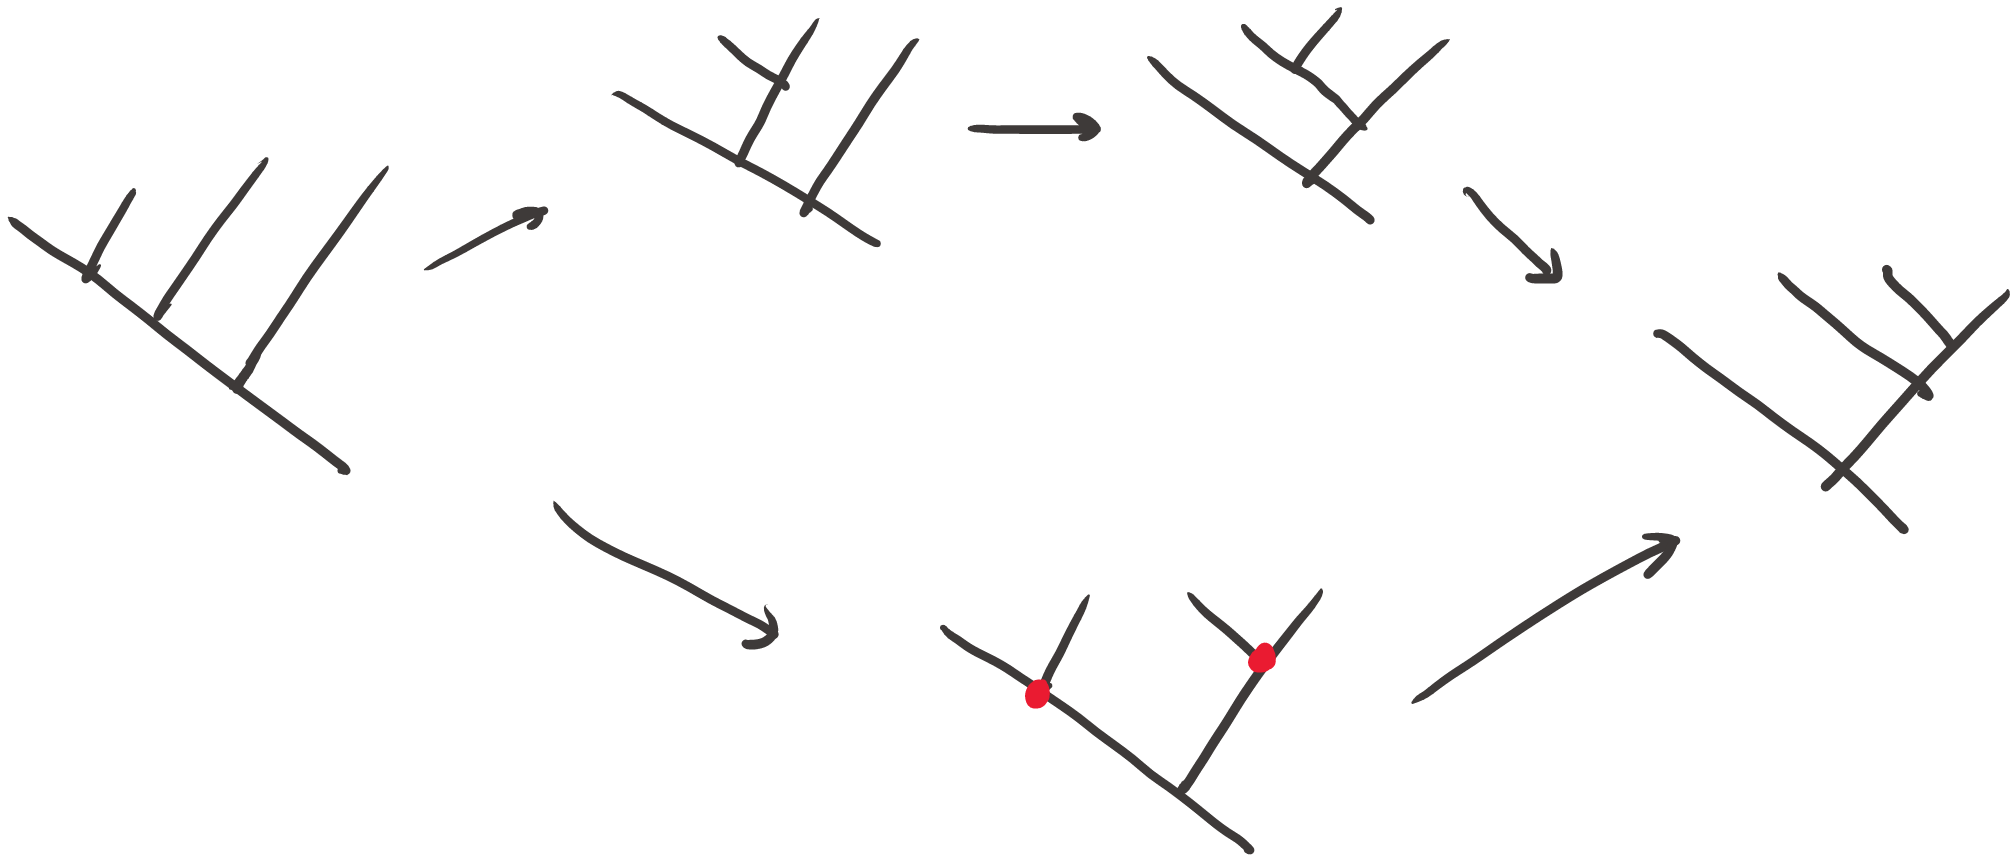
\includegraphics[height=3cm]{pentagon}        
    \end{center}
    \item Bosonic SPT: $d\nu_3=0$;
    \item Fermionic SPT:
    \[d\nu_3(g1, g2, g3, g4)=O_4[n_2](g1, g2, g3, g4)=\frac12 n_2(g1, g2) n_2(g3, g4) + \cdots\]
  \end{itemize}
\end{frame}

\begin{frame}{Construction of fSPT states}
  \begin{enumerate}
  \item Pick $n_1\in H^1(G, \mathbb Z_2)$.
  \item Compute $O_3[n_1]\in H^3(G, \mathbb Z_2)$ and see if it is trivial.
  \item Solve $dn_2 = O_3[n_1]$ (pick a $n_2$).
  \item Compute $O_4[n_2]\in H^4[G, \mathrm U(1)_T]$ and see if it is trivial.
  \item Solve $d\nu_3 = O_4[n_2]$.
  \end{enumerate}
\end{frame}

\begin{frame}
  \frametitle{Stacking operation}
  \begin{itemize}
  \item Not a simple component-wise addition:
    $(n_1,n_2,\nu_3)\boxplus(n_1',n_2',\nu_3')\neq (n_1+n_1',n_2+n_2',\nu_3+\nu_3')$.
  \item Reason: reordering of fermionic degrees of freedom.
  \item Result on the $p$-th layer will be twisted by higher layers.
  \item Examples: in 2d, $G=G_b\times\mathbb Z_2^f$
    \begin{align*}
      \Delta n_2 &= n_1\cup n_1';\\
      \Delta \nu_3 &= \frac12n_2\cup_1n_2' + \cdots.
    \end{align*}
  \end{itemize}
  \begin{center}
    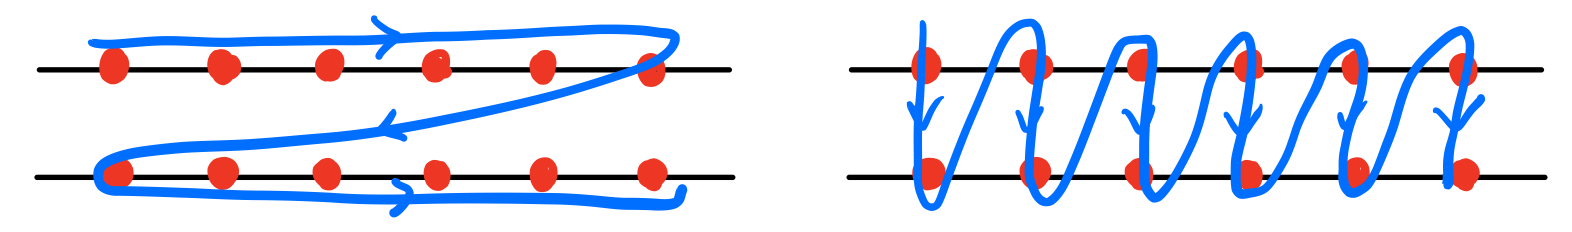
\includegraphics[height=2cm]{../chainmap/forder}
  \end{center}
\end{frame}

\begin{frame}
  \frametitle{Simplified resolution and chain maps}
  \begin{itemize}
  \item A problem: cochains $\alpha(g_1,\ldots,g_n)$ are too complicated to deal with.
    \begin{itemize}
    \item $\alpha: [g_1|\cdots|g_n]\rightarrow M$ is a ``linear map''.
    \item $d\alpha = O_{n+1}$: like solving a ``linear equation''. 
    \item Complexity: $O(N^3)$;
    \item Traditionally: $N=(|G|-1)^{d+1}$; very expensive if $d$ and $G$ is large.
    \end{itemize}
  \item A simplified resolution: a simplified basis replacing $[g_1|\cdots|g_n]$.
  \item $N<100$ for all space groups.
  \item Chain maps: a ``compiler'' converting formulas from the standard basis to the simplified basis.
  \item Allows computation for infinite (discrete) groups.
  \item Yunqing Ouyang, Qing-Rui Wang, Zheng-Cheng Gu and YQ,\\ Chin. Phys. Lett. \textbf{38} 127101 (2021).
  \end{itemize}
\end{frame}

\begin{frame}[fragile]{SptSet: a GAP Package}
	\begin{itemize}
		\item Computes fSPT classification.
		\item Available at \url{https://github.com/yangqi137/SptSet}.
		\item Obstruction functions are included.
    \[O_3[n_1]=s\cup n_1\cup c_1.\]
    \begin{lstlisting}[basicstyle=\footnotesize]
      SptSetInstallCoboundary(ss, 2, 1, 2,
      function(n1, dn1)
        return {g1, g2, g3} -> (s(g1) * n1(g2) * n1(g3));
      end);
      \end{lstlisting}
		\item Battery included in \lstinline|SptSet|: construction of $\omega_2^{s=1/2}$ for 2d and 3d space groups
    \begin{lstlisting}[basicstyle=\footnotesize]
    w2 := Spin12Factor(d, it);
    \end{lstlisting}
		\item Will be improved in the future.
	\end{itemize}
\end{frame}

\begin{frame}[fragile]{Example: fSPT for 2D wallpaper groups}
	\url{SptSet/examples/fspt_2d_s12.g}
	\begin{lstlisting}[basicstyle=\footnotesize]
    for it in [2..17] do
      SG := SpaceGroupBBNWZ(2, it);
      fSG := IsomorphismPcpGroup(SG);
      SG1 := Image(fSG);
      R := ResolutionAlmostCrystalGroup(SG1, 6);
      gs := GeneratorsOfGroup(SG);
      w := Spin12Factor(2, it);
      ww := {g1, g2} -> w(PreImageElm(fSG, g1), PreImageElm(fSG, g2));
      f := GroupHomomorphismByImagesNC(SG1, GL(1, Integers),
        List(gs, x -> Image(fSG, x)),
        List(gs, x -> [[DeterminantMat(x)]]));

      SS := FermionSPTSpecSeq(R, f, ww);
      FermionSPTLayersVerbose(SS, 2);
    od;
  \end{lstlisting}
  17 wallpaper groups in ~6 minutes.
\end{frame}

\begin{frame}{Current status}
  \begin{itemize}
    \item 2d fSPT: all solved.
    \begin{itemize}
      \item Formulas for the obstruction functions: QR Wang and ZC Gu, PRX 10, 031055 (2020).
      \item Formulas for stacking: Xing-Yu Ren et al, arXiv:2310.19058.
      \item SptSet package can reproduce the results of real-space construction by JH Zhang, et al.
    \end{itemize}
    \item 3d fSPT: work in progress.
    \begin{itemize}
      \item Formulas for the obstruction functions: Shang-Qiang Ning, et al, to appear.
      \item Stacking?
      \item SptSet package: work in progress.
    \end{itemize}
  \end{itemize}
\end{frame}

\begin{frame}{Other tasks}
	\begin{enumerate}
		\item TIs: interacting fSPT with U(1) symmetry.
		\begin{itemize}
			\item Given $1\rightarrow U(1)_f\rightarrow G_f\rightarrow G\rightarrow 1$, we have
			\[E_2^{pq}=H^p(G, \mathcal H^q(U(1)))\Rightarrow \mathcal H^{p+q}(G_f).\]
      \item Decorating U(1)-SPTs: $\mathcal H^1(U(1))=\mathbb Z$ (charge);\\ $\mathcal H^2(U(1))=0$;
        $\mathcal H^3((U(1)))=\mathbb Z$ (Chern insulator).
			\item Jian-Hao Zhang, et al, PRResearch \textbf{4}, 033081 (2022).
			\item Can be computed using the \lstinline|InsulatorSPTSpecSeq| function.
		\end{itemize}

		\item ASPTs:
		\begin{itemize}
			\item $G_b$ is averaged symmetry, $\mathbb Z_2^f$ is exact.
			\item Remove the bSPT layer: $\mathcal H^0_A(*)=0$ in $E_2^{pq}=H^p(G_b, \mathcal H^q_A(*))$.
			\item Can be computed using the \lstinline|AvgFermionSPTSpecSeq| function.
		\end{itemize}
	\end{enumerate}
\end{frame}

% \subsection{Free-fermion SPTs}

% \begin{frame}{Free-fermion: K-theory classification}
%   \begin{columns}
%     \column{.4\textwidth}
%     \begin{itemize}
%       \item 10-fold way and Bott periodicity.
%       \item Atiyah-Bott-Shapiro construction:
%       \[H=iM_0+\sum_ik_i\Gamma_i;\]
%       \item Clifford Algebra: $\mathrm{Cl}^{q+1, d}$ or $\mathbb C\mathrm l^{q+1+d}$
%       \item Classification: whether we can find another mass term?
%     \end{itemize}
%     \column{.6\textwidth}{\small
%     \begin{tabular}{c|ccc|cc|cccc}
%       \hline
%       Class & $T^2$ & $C^2$ & $S$ & Type & q & 0d & 1d & 2d & 3d\\
%       \hline\hline
%       A & 0 & 0 & 0 & $\mathbb C$ & 0 & $\mathbb Z$ & 0 & $\mathbb Z$ & 0\\
%       AIII & 0&0&1 & $\mathbb C$&1 & 0 & $\mathbb Z$ & 0 & $\mathbb Z$\\
%       \hline
%       D & 0&+1&0 & $\mathbb R$&0 & $\mathbb Z_2$&$\mathbb Z_2$&$\mathbb Z$&0\\
%       DIII & $-1$&+1&1 & $\mathbb R$&1 & 0&$\mathbb Z_2$&$\mathbb Z_2$&$\mathbb Z$\\
%       AII & $-1$&0&0 & $\mathbb R$&2 & $\mathbb Z$&0&$\mathbb Z_2$&$\mathbb Z_2$\\
%       CII & $-1$&$-1$&1 & $\mathbb R$&3 & 0&$\mathbb Z$&0&$\mathbb Z_2$\\
%       C & 0&$-1$&0 & $\mathbb R$&4 & 0&0&$\mathbb Z$&0\\
%       CI & +1&$-1$&1 & $\mathbb R$&5 & 0&0&0&$\mathbb Z$\\
%       AI & +1&0&0 & $\mathbb R$&6 & $\mathbb Z$&0&0&0\\
%       BDI & +1&+1&1 & $\mathbb R$&7 & $\mathbb Z_2$&$\mathbb Z$&0&0\\
%       \hline
%     \end{tabular}}
%   \end{columns}
% \end{frame}

\section{Approach II: real-space construction}

\begin{frame}
	\frametitle{Decomposition of the space}
	We divide the space into \alert{finer cells} such that there's \alert{only onsite symmetry} on each cell.
	\begin{enumerate}
		\item A cell $\sigma$ is maped to one single cell $\sigma^\prime$ under $SG$-action.
		\item $G_\sigma=\{g\in G|g:\sigma\rightarrow\sigma\}$ acts on $\sigma$ as onsite symmetry.
		\item A proper $G$-complex $Y\simeq \mathbb R^d$.
	\end{enumerate}
	\begin{columns}
		\column{.5\textwidth}
		\begin{center}
			\includegraphics[width=.5\textwidth]{../spspt/blocks}
		\end{center}
		\column{.5\textwidth}
		\begin{center}
			\begin{tikzpicture}
				\draw (-2, -2)--(-2, 2)--(2, 2)--(2, -2)--(-2, -2);
				\draw<2> [thick] (0, -2)--(0, 2);
				\draw [->] (.7, 0) arc (0:180:0.7);
				\filldraw (0, 0) circle (1pt) node [right] {$C_2$};
				\node<2> at (0, -1) [right] {$\tau_1$};
				\node<2> at (0, 1) [left] {$\tau_2$};
				\node<2> at (-1, 0) {$\sigma_1$};
				\node<2> at (1, 0) {$\sigma_2$};
			\end{tikzpicture}
		\end{center}
	\end{columns}
\end{frame}

\begin{frame}
	\frametitle{Topological crystalline states are made of building blocks}
	\begin{columns}
		\column{.4\textwidth}
		\begin{center}
			\includegraphics[width=\textwidth]{../spspt/blocks}
		\end{center}
		\column{.6\textwidth}
		\begin{itemize}
			\item We divide the space into cells compatible with the space-group symmetry.
			\item On a $p$-cell $\sigma$, the SPT state is protected only by $G_\sigma$.
			\[\hat\omega(\sigma)\in \Phi^p(G_\sigma) = H^{p+1}[G_\sigma,\uone_T].\]
			\item $G_\sigma$ acts as onsite symmetries.
			\item Decorate 3d SPT on 3-cells; 2d SPT on 2-cells; 1d SPT on 1-cells; 0d SPT on 0-cells;
			\item $p$-block states: $E^p_{p,\infty}$.
			\[\text{TCSs} = ``\bigoplus_p\text{''} E^p_{p,\infty}.\]
		\end{itemize}
	\end{columns}
\end{frame}

\begin{frame}
	\frametitle{Symmetric conditions}
	\begin{columns}
		\column{.3\textwidth}
		\begin{tikzpicture}
			\draw (0, 0)--(2, 0)--(2, 2)--(0, 2)--(0, 0);
			\draw (2, 4)--(4, 4)--(4, 6)--(2, 6)--(2, 4);
			\draw [thick,->] (1, 1) node [below] {$\hat\omega(\sigma$)} --
			(3, 5) node [above] {$\hat\omega(\sigma^\prime)$};
			\node at (2, 3) [right] {$g$};
		\end{tikzpicture}
		\column{.7\textwidth}
		\begin{itemize}
			\item If $g:\sigma\rightarrow\sigma^\prime$, then the cochains attached must be ``identical''.
			\item $G_\sigma\neq G_{\sigma'}$, but they are isomorphic:
			\[G_{\sigma'}=gG_\sigma g^{-1}\simeq G_\sigma.\]
			\item This induces another isomorphism:
			\[H^{p+1}[G_{\sigma'},\uone_T]\simeq H^{p+1}[G_\sigma,\uone_T]\]
			\item $\hat\omega(\sigma)$ and $\hat\omega(\sigma')$ are related by this isomorphism
			\[\hat\omega(\sigma') = g\cdot \hat\omega(\sigma).\]
			\item Only decorations on symmetry-unrelated cells are independent: finite \# of them.
		\end{itemize}
	\end{columns}
\end{frame}

\begin{frame}
	\frametitle{No-Open-Edge Conditions}
	\begin{columns}
		\column{.58\textwidth}
		\begin{itemize}
			\item<1-> SPT blocks have nontrivial boundary states.
			\item<2-> Boundary anomaly must cancel on $(p-1)$-cells.
			\item<3-> $\hat\omega(\sigma_1)
			+\hat\omega(\sigma_2)+\hat\omega(\sigma_3)+\hat\omega(\sigma_4)\simeq0$.
		\end{itemize}
		\column{.42\textwidth}
		\begin{tikzpicture}
			\draw (0, 1)--(-1, 1)--(-2, 0)--(2, 0)--(3, 1)--(1, 1);
			\draw [thick] (0, 0)--(1, 1);
			\draw<1-2> [string] (.2, .1)--(1, .9);
			\draw<1> [string] (1, .9)--(2.8, .9);
			\draw<1> [string] (2.8, .9)--(2, .1);
			\draw<1> [string] (2, .1)--(.2, .1);
			\draw<2> [string] (.1, .2)--(.9, 1);
			\draw<3-> [->] (1.3, .5)--(.6, .5);
			\draw<3-> [->] (.5, 1.3)--(.5, .6);
			\draw<3-> [->] (.5, -.3)--(.5, .4);
			\draw<3-> [->] (-.3, .5)--(.4, .5);
			\node<1-2> at (.5, .5) [above] {$\tau$};
			\node<3-> at (.7, .7) [above] {$\tau$};
			\draw (1, 1)--(1, 3)--(0, 2)--(0, -2)--(0, -2)--(1, -1)--(1, 0);
			\node at (.5, 1.5) {$\sigma_1$};
			\node at (1.5, .5) {$\sigma_2$};
			\node at (.5, -0.5) {$\sigma_3$};
			\node at (-0.5, .5) {$\sigma_4$};
		\end{tikzpicture}
	\end{columns}
\end{frame}

\begin{frame}
	\frametitle{Bubbling Equivalence}
\begin{columns}
\column{.7\textwidth}
\begin{itemize}
\item A bubbling process: fill a 2-cell with a loop of 1-dim SPT states.
\item Changes 1-cell decoration.
\item Does not change bulk classification.
\item Two decorations should be viewed as equivalent ones.
\end{itemize}
\column{.3\textwidth}
\begin{animateinline}{5}
        \multiframe{12}{Ra=.3+.05}{
\begin{tikzpicture}[scale=1]
	\draw (0, 0)--(2, 0)--(2, 2)--(0, 2)--(0, 0);
	\draw [dashed] (1, 2)--(1, 1)--(2, 1);
	\draw (2, 1)--(3, 1)--(3, 3)--(1, 3)--(1, 2);
	\draw [dashed] (0, 0)--(1, 1);
	\draw (2, 0)--(3, 1);
	\draw (0, 2)--(1, 3);
	\draw (2, 2)--(3, 3);
	\fill [blue!30,opacity=.5] (1.5-1.5*\Ra, 1.5-1.5*\Ra)--(1.5+0.5*\Ra, 1.5-1.5*\Ra)
	--(1.5+1.5*\Ra, 1.5-0.5*\Ra)--(1.5+1.5*\Ra, 1.5+1.5*\Ra)
	--(1.5-0.5*\Ra, 1.5+1.5*\Ra)--(1.5-1.5*\Ra, 1.5+0.5*\Ra)
	--(1.5-1.5*\Ra, 1.5-1.5*\Ra);
	\draw [blue,dashed] (1.5-1.5*\Ra, 1.5+0.5*\Ra)--(1.5+0.5*\Ra, 1.5+0.5*\Ra)--(1.5+1.5*\Ra,1.5+1.5*\Ra);
	\draw [blue,dashed] (1.5+0.5*\Ra, 1.5-1.5*\Ra)--(1.5+0.5*\Ra, 1.5+0.5*\Ra);
	\draw [->,thick] (1.5-0.5*\Ra, 1.5-0.5*\Ra)--(1.3-0.5*\Ra, 1.3-0.5*\Ra);
	\draw [->,thick] (1.5, 1.5+\Ra)--(1.5, 1.78+\Ra);
	\draw [->,thick] (1.5+\Ra, 1.5)--(1.78+\Ra, 1.5);
	%\fill [green!30] (-\Ra,-\Ra)--(-\Ra,\Ra)--(\Ra,\Ra)--(\Ra,-\Ra)--(-\Ra,-\Ra);
%\draw [blue,thick] (-\Ra,-\Ra)--(-\Ra,\Ra)--(\Ra,\Ra)--(\Ra,-\Ra)--(-\Ra,-\Ra);
%\node at (0, 0) {$d\nu$};
\end{tikzpicture}
}
\end{animateinline}
\end{columns}
\end{frame}

\begin{frame}
  \frametitle{2nd page: a homology-group calculation}
  \begin{itemize}
  \item No-open-edge conditions:
    \[d_1\hat\omega\simeq 0, \hat\omega\in E^p_{p,1}.\]
  \item Bubbling equivalence:
    \[d_1\hat\mu\simeq 0, \hat\mu\in E^p_{p+1,1}.\]
  \item A homology-group calculation:
    \[E^p_{p+1,1}\xrightarrow{d_1}E^p_{p,1}\xrightarrow{d_1}E^p_{p-1,1},\]
    \[E^p_{p,2}=\frac{\ker d^p_{p,1}}{\img d^p_{p+1,1}}.\]
  \end{itemize}
\end{frame}

\begin{frame}
  \frametitle{Cases when the second page is enough}
  \begin{itemize}
  \item If $G = SG\times G_0$.
  \item If we ignore $\Omega_0$: not treating the atomic insulators as nontrivial SPTs.
  \item Only need to compute the second page:
    \begin{enumerate}
    \item $E^2_{2,2}$: assign 2d SPTs to 2-cells, and check-anomaly vanishing on 1-cells. Coboundaries are assigning 2d SPTs to 3-cells.
    \item $E^1_{1,2}$: assign 1d SPTs to 1-cells, and check-anomaly vanishing on 0-cells. Coboundaries are assigning 1d SPTs to 2-cells.
    \end{enumerate}
  \item Trivial group extension: $E^2_{2,2}\oplus E^1_{1,2}$.
  \end{itemize}
\end{frame}

%\section{Recipe: higher pages}

\begin{frame}
\frametitle{General construction: a ``perturbative'' approach}
We can classify building blocks according to the leading dimension:
\begin{align*}
E^3_{3,\infty}:\hat\omega_{3+}&= \alert{\hat\omega_3} + \hat\omega_2+ \hat\omega_1+ \hat\omega_0;\\
E^2_{2,\infty}:\hat\omega_{2+}&= \alert{\hat\omega_2}+ \hat\omega_1+ \hat\omega_0;\\
E^1_{1,\infty}:\hat\omega_{1+}&= \alert{\hat\omega_1}+ \hat\omega_0;\\
E^0_{0,\infty}:\hat\omega_{0+}&= \alert{\hat\omega_0};
\end{align*}
\begin{itemize}
\item We only choose a special solution for subleading terms.
\item Need to know the precise wave function: more about cohomology theory...

\item \alert{Building blocks} / Connectors.
\end{itemize}
\begin{center}
\begin{tikzpicture}[scale=1.5]
\fill [blue!50] (0.1,0.1)--(1,0.1)--(1.4,.5)--(1.4,1.4)--(0.5,1.4)--(.1,1)--(0.1,0.1);
\draw (0,0)--(1,0)--(1,1)--(0,1)--(0,0);
\draw (1,0)--(1.5,.5)--(1.5,1.5)--(1,1);
\draw (1.5,1.5)--(0.5,1.5)--(0,1);
\end{tikzpicture}~~~~
\begin{tikzpicture} [scale=1.5]
\fill [blue!50] (0,0)--(1,0)--(1.5,.5)--(1.5,1.5)--(0.5,1.5)--(0,1)--(0,0);
\draw (0,0)--(1,0)--(1,1)--(0,1)--(0,0);
\draw (1,0)--(1.5,.5)--(1.5,1.5)--(1,1);
\draw (1.5,1.5)--(0.5,1.5)--(0,1);
\draw (0,0)--(.5,.5)--(.5,1.5);
\draw (.5,.5)--(1.5,.5);
\end{tikzpicture}~~~~
\begin{tikzpicture} [scale=1.5]
\draw [thick,blue] (0,0)--(1,0)--(1,1)--(0,1)--(0,0);
\draw [thick,blue](1,0)--(1.5,.5)--(1.5,1.5)--(1,1);
\draw [thick,blue](1.5,1.5)--(0.5,1.5)--(0,1);
\draw [thick,blue](0,0)--(.5,.5)--(.5,1.5);
\draw [thick,blue](.5,.5)--(1.5,.5);
\end{tikzpicture}~~~~
\begin{tikzpicture} [scale=1.5]
\draw (0,0)--(1,0)--(1,1)--(0,1)--(0,0);
\draw (1,0)--(1.5,.5)--(1.5,1.5)--(1,1);
\draw (1.5,1.5)--(0.5,1.5)--(0,1);
\draw (0,0)--(.5,.5)--(.5,1.5);
\draw (.5,.5)--(1.5,.5);
\filldraw [blue] (0,0) circle (2pt);
\filldraw [blue] (1,0) circle (2pt);
\filldraw [blue] (0,1) circle (2pt);
\filldraw [blue] (1,1) circle (2pt);
\filldraw [blue] (0.5,0.5) circle (2pt);
\filldraw [blue] (0.5,1.5) circle (2pt);
\filldraw [blue] (1.5,0.5) circle (2pt);
\filldraw [blue] (1.5,1.5) circle (2pt);
\end{tikzpicture}
\end{center}
\end{frame}

\begin{frame}
\frametitle{High-Order No-Open-Edge Conditions}
\begin{columns}
\column{.6\textwidth}
\begin{enumerate}
\item<1-> Choose a cocycle for each 2-cell $\sigma$.\\ Check $\partial\hat\omega_2(\tau)\simeq0$ for each 1-cell $\tau$.\\
\emph{1st-page no-open-edge condition.}
\item<2-> Choose a cochain $\hat\omega_1$ for each $\tau$.\\
Check $\partial\hat\omega_1(\lambda)\simeq0$ for each 0-cell $\lambda$.\\
\emph{2nd-page no-open-edge condition.}
\item<3> Choose a cochain $\hat\omega_0$ for each $\lambda$.
\end{enumerate}
\column{.4\textwidth}
\begin{center}
\begin{tikzpicture} [scale=3]
\fill [blue!50] (0,0)--(1,0)--(1.5,.5)--(1.5,1.5)--(0.5,1.5)--(0,1)--(0,0);
\draw<1> [thick,white] (0,0)--(1,0)--(1,1)--(0,1)--(0,0);
\draw<1> [thick,white] (1,0)--(1.5,.5)--(1.5,1.5)--(1,1);
\draw<1> [thick,white] (1.5,1.5)--(0.5,1.5)--(0,1);
\draw<1> [thick,white] (0,0)--(.5,.5)--(.5,1.5);
\draw<1> [thick,white](.5,.5)--(1.5,.5);
\draw<2-> [thick,red] (0,0)--(1,0)--(1,1)--(0,1)--(0,0);
\draw<2-> [thick,red] (1,0)--(1.5,.5)--(1.5,1.5)--(1,1);
\draw<2-> [thick,red] (1.5,1.5)--(0.5,1.5)--(0,1);
\draw<2-> [thick,red] (0,0)--(.5,.5)--(.5,1.5);
\draw<2-> [thick,red](.5,.5)--(1.5,.5);
\fill<1-2> [white] (0,0) circle (2pt);
\fill<1-2> [white] (1,0) circle (2pt);
\fill<1-2> [white] (0,1) circle (2pt);
\fill<1-2> [white] (1,1) circle (2pt);
\fill<1-2> [white] (0.5,0.5) circle (2pt);
\fill<1-2> [white] (1.5,0.5) circle (2pt);
\fill<1-2> [white] (0.5,1.5) circle (2pt);
\fill<1-2> [white] (1.5,1.5) circle (2pt);
\fill<3> [red] (0,0) circle (2pt);
\fill<3> [red] (1,0) circle (2pt);
\fill<3> [red] (0,1) circle (2pt);
\fill<3> [red] (1,1) circle (2pt);
\fill<3> [red] (0.5,0.5) circle (2pt);
\fill<3> [red] (1.5,0.5) circle (2pt);
\fill<3> [red] (0.5,1.5) circle (2pt);
\fill<3> [red] (1.5,1.5) circle (2pt);
\end{tikzpicture}
\end{center}
\end{columns}
\end{frame}

\begin{frame}
\frametitle{High-Order Bubbling Equivalences}
\begin{itemize}
\item Similarly, there are high-order bubbling equivalence.
\item Assign 1d SPT states ($d\hat\mu_1=0$) to 2-cells: $\partial\hat\mu_2$ trivializes $\hat\omega_1$ building blocks.
\item If $\partial\hat\mu_2\simeq0$, choose $d\hat\mu_1+\partial\hat\mu_2=0$, then $\partial\hat\mu_1$ trivializes $\hat\omega_0$ building blocks.
\item High-order computations are organized as a \alert{spectral sequence}.
\end{itemize}
\begin{center}
\begin{animateinline}{5}
        \multiframe{12}{Ra=.4+.05}{
\begin{tikzpicture}
	\draw (-2,-2)--(-2,2)--(2,2)--(2,-2)--(-2,-2);
   \draw (-2,0)--(2,0);
   \draw (0,-2)--(0,2);
	%\fill [green!30] (-\Ra,-\Ra)--(-\Ra,\Ra)--(\Ra,\Ra)--(\Ra,-\Ra)--(-\Ra,-\Ra);
\draw [blue,thick] (-\Ra+1,-\Ra+1)--(-\Ra+1,\Ra+1)--(\Ra+1,\Ra+1)--(\Ra+1,-\Ra+1)--(-\Ra+1,-\Ra+1);
\draw [blue,thick] (-\Ra+1,-\Ra-1)--(-\Ra+1,\Ra-1)--(\Ra+1,\Ra-1)--(\Ra+1,-\Ra-1)--(-\Ra+1,-\Ra-1);
\draw [blue,thick] (-\Ra-1,-\Ra+1)--(-\Ra-1,\Ra+1)--(\Ra-1,\Ra+1)--(\Ra-1,-\Ra+1)--(-\Ra-1,-\Ra+1);
\draw [blue,thick] (-\Ra-1,-\Ra-1)--(-\Ra-1,\Ra-1)--(\Ra-1,\Ra-1)--(\Ra-1,-\Ra-1)--(-\Ra-1,-\Ra-1);
%\node at (0, 0) {$d\nu$};
%\node at (\Ra, 0) [left] {$\nu$};
\end{tikzpicture}
}
\end{animateinline}
~~~~
\begin{animateinline}{5}
        \multiframe{8}{Ra=.8+-.1}{
\begin{tikzpicture}
\draw (-2,0)--(2,0);
\draw (0, -2)--(0, 2);
\draw [blue,thick,double] (-\Ra, 0)--(\Ra,0);
\draw [blue,thick,double] (2-\Ra,0)--(2,0);
\draw [blue,thick,double] (-2+\Ra,0)--(-2,0);
\draw [blue,thick,double] (0, -\Ra)--(0, \Ra);
\draw [blue,thick,double] (0, 2-\Ra)--(0, 2);
\draw [blue,thick,double] (0, -2+\Ra)--(0, -2);
\fill [red] (-\Ra,0) circle (2pt);
\fill [red] (\Ra,0) circle (2pt);
\fill [red] (0,-\Ra) circle (2pt);
\fill [red] (0,\Ra) circle (2pt);
\fill [red] (2-\Ra,0) circle (2pt);
\fill [red] (-2+\Ra,0) circle (2pt);
\fill [red] (0,2-\Ra) circle (2pt);
\fill [red] (0,-2+\Ra) circle (2pt);
\end{tikzpicture}
}
\end{animateinline}
\end{center}
\end{frame}
\begin{frame}
  \frametitle{A spectral sequence}
  We compute in the following sequence:
  \begin{enumerate}
  \item 0st-page no-open-edge condition + 0st-page bubbling equivalence.
  \[E^p_{p,1}=\frac{\ker d_0}{\img d_0}.\]
  \item 1st-page no-open-edge condition + 0st-page bubbling equivalence.
  \[E^p_{p,2}=\frac{\ker d_1}{\img d_1}.\]
  \item 2nd-page no-open-edge condition + 0st-page bubbling equivalence.
  \[E^p_{p,3}=\frac{\ker d_2}{\img d_2}.\]
  \end{enumerate}
  
  \[E^p_{p,1}\supseteq E^p_{p,2}\supseteq E^p_{p,3}\supseteq\cdots=E^p_{p,\infty}.\]
  \end{frame}
  
  \begin{frame}
  \frametitle{First Page}
  \begin{center}
  \begin{tikzpicture}
  \draw (0,0)--(4,0)--(4,2)--(0,2)--(0,0);
  \node at (2,1) {$\hat\omega(\sigma)$};
  \end{tikzpicture}
  \end{center}
  \begin{itemize}
  \item The first page concerns only the building blocks.
  \item $d\hat\omega(\sigma)=0$.
  \item $d\hat\mu(\sigma)\sim0$.
  \item Define $d_0=d$.
  \end{itemize}
  \[E^p_{p,1}=\frac{\ker d_0}{\img d_0}
  =\bigoplus_{\sigma\in Y_p/G}H^p(G_\sigma, U(1)_T).\]
  \end{frame}
  
  \begin{frame}
  \frametitle{Second Page}
  \begin{center}
      \begin{tikzpicture}[scale=.6]
        \draw (0, 1)--(-1, 1)--(-2, 0)--(2, 0)--(3, 1)--(1, 1);
        \draw [thick] (0, 0)--(1, 1);
        \node at (.5, .5) [above] {$\tau$};
        \draw (1, 1)--(1, 3)--(0, 2)--(0, -2)--(0, -2)--(1, -1)--(1, 0);
        \node at (.5, 1.5) {$\sigma_1$};
        \node at (1.5, .5) {$\sigma_2$};
        \node at (.5, -0.5) {$\sigma_3$};
        \node at (-0.5, .5) {$\sigma_4$};
      \end{tikzpicture}
  ~~~~
  \begin{animateinline}{5}
          \multiframe{12}{Ra=.4+.05}{
  \begin{tikzpicture}[scale=.6]
    \draw (-2,-2)--(-2,2)--(2,2)--(2,-2)--(-2,-2);
     \draw (-2,0)--(2,0);
     \draw (0,-2)--(0,2);
    %\fill [green!30] (-\Ra,-\Ra)--(-\Ra,\Ra)--(\Ra,\Ra)--(\Ra,-\Ra)--(-\Ra,-\Ra);
  \draw [blue,thick] (-\Ra+1,-\Ra+1)--(-\Ra+1,\Ra+1)--(\Ra+1,\Ra+1)--(\Ra+1,-\Ra+1)--(-\Ra+1,-\Ra+1);
  \draw [blue,thick] (-\Ra+1,-\Ra-1)--(-\Ra+1,\Ra-1)--(\Ra+1,\Ra-1)--(\Ra+1,-\Ra-1)--(-\Ra+1,-\Ra-1);
  \draw [blue,thick] (-\Ra-1,-\Ra+1)--(-\Ra-1,\Ra+1)--(\Ra-1,\Ra+1)--(\Ra-1,-\Ra+1)--(-\Ra-1,-\Ra+1);
  \draw [blue,thick] (-\Ra-1,-\Ra-1)--(-\Ra-1,\Ra-1)--(\Ra-1,\Ra-1)--(\Ra-1,-\Ra-1)--(-\Ra-1,-\Ra-1);
  %\node at (0, 0) {$d\nu$};
  %\node at (\Ra, 0) [left] {$\nu$};
  \end{tikzpicture}
  }
  \end{animateinline}
  \end{center}
  \begin{itemize}
  \item No-open-edge condition: $\partial\hat\omega_2\sim0$.
  \item Bubbling equivalence: $\hat\omega_2\rightarrow\hat\omega_2+\partial\hat\mu_3$.
  \item Define $d_1=\partial:E^q_{p,1}\rightarrow E^q_{p-1,1}$.
  \end{itemize}
  \[E^p_{p,2}=\frac{\ker d_1}{\img d_1}.\]
  \end{frame}
  
  \begin{frame}
  \frametitle{Third Page}
  \begin{center}
  \begin{tikzpicture} [scale=1.5]
  \fill [blue!50] (0,0)--(1,0)--(1.5,.5)--(1.5,1.5)--(0.5,1.5)--(0,1)--(0,0);
  \draw [thick,black!50!green] (0,0)--(1,0)--(1,1)--(0,1)--(0,0);
  \draw [thick,thick,black!50!green] (1,0)--(1.5,.5)--(1.5,1.5)--(1,1);
  \draw [thick,thick,black!50!green] (1.5,1.5)--(0.5,1.5)--(0,1);
  \draw [thick,thick,black!50!green] (0,0)--(.5,.5)--(.5,1.5);
  \draw [thick,thick,black!50!green](.5,.5)--(1.5,.5);
  \fill [red] (0,0) circle (2pt);
  \fill [red] (1,0) circle (2pt);
  \fill [red] (0,1) circle (2pt);
  \fill [red] (1,1) circle (2pt);
  \fill [red] (0.5,0.5) circle (2pt);
  \fill [red] (1.5,0.5) circle (2pt);
  \fill [red] (0.5,1.5) circle (2pt);
  \fill [red] (1.5,1.5) circle (2pt);
  \end{tikzpicture}
  ~~~~
  \begin{animateinline}{5}
          \multiframe{12}{Ra=.4+.05}{
  \begin{tikzpicture}[scale=.6]
    \draw (-2,-2)--(-2,2)--(2,2)--(2,-2)--(-2,-2);
     \draw (-2,0)--(2,0);
     \draw (0,-2)--(0,2);
    %\fill [green!30] (-\Ra,-\Ra)--(-\Ra,\Ra)--(\Ra,\Ra)--(\Ra,-\Ra)--(-\Ra,-\Ra);
  \draw [blue,thick] (-\Ra+1,-\Ra+1)--(-\Ra+1,\Ra+1)--(\Ra+1,\Ra+1)--(\Ra+1,-\Ra+1)--(-\Ra+1,-\Ra+1);
  \draw [blue,thick] (-\Ra+1,-\Ra-1)--(-\Ra+1,\Ra-1)--(\Ra+1,\Ra-1)--(\Ra+1,-\Ra-1)--(-\Ra+1,-\Ra-1);
  \draw [blue,thick] (-\Ra-1,-\Ra+1)--(-\Ra-1,\Ra+1)--(\Ra-1,\Ra+1)--(\Ra-1,-\Ra+1)--(-\Ra-1,-\Ra+1);
  \draw [blue,thick] (-\Ra-1,-\Ra-1)--(-\Ra-1,\Ra-1)--(\Ra-1,\Ra-1)--(\Ra-1,-\Ra-1)--(-\Ra-1,-\Ra-1);
  %\node at (0, 0) {$d\nu$};
  %\node at (\Ra, 0) [left] {$\nu$};
  \end{tikzpicture}
  }
  \end{animateinline}
  ~~~~
  \begin{animateinline}{5}
          \multiframe{8}{Ra=.8+-.1}{
  \begin{tikzpicture}[scale=.6]
  \draw (-2,0)--(2,0);
  \draw (0, -2)--(0, 2);
  \draw [blue,thick,double] (-\Ra, 0)--(\Ra,0);
  \draw [blue,thick,double] (2-\Ra,0)--(2,0);
  \draw [blue,thick,double] (-2+\Ra,0)--(-2,0);
  \draw [blue,thick,double] (0, -\Ra)--(0, \Ra);
  \draw [blue,thick,double] (0, 2-\Ra)--(0, 2);
  \draw [blue,thick,double] (0, -2+\Ra)--(0, -2);
  \fill [red] (-\Ra,0) circle (2pt);
  \fill [red] (\Ra,0) circle (2pt);
  \fill [red] (0,-\Ra) circle (2pt);
  \fill [red] (0,\Ra) circle (2pt);
  \fill [red] (2-\Ra,0) circle (2pt);
  \fill [red] (-2+\Ra,0) circle (2pt);
  \fill [red] (0,2-\Ra) circle (2pt);
  \fill [red] (0,-2+\Ra) circle (2pt);
  \end{tikzpicture}
  }
  \end{animateinline}
  \end{center}
  \begin{itemize}
  \item Define $d_2:E^q_{p,2}\rightarrow E^{q-1}_{p-2,2}$:
  \begin{enumerate}
  \item Start from $\hat\omega_p$.
  \item Find the connectors $\hat\omega_{p-1}$, s.t. $d\hat\omega_{p-1}=\partial\hat\omega_p$.
  \item Compute $d_2\hat\omega_p=\partial\hat\omega_{p-1}$.
  \end{enumerate}
  \item No-open-edge condition: $d_2\hat\omega_p\sim0$.
  \item Bubbling equivalence: $\hat\omega_p\rightarrow\hat\omega_p+d_2\hat\omega_{p+2}$.
  \end{itemize}
  \[E^p_{p,3}=\frac{\ker d_2}{\img d_2}.\]
  \end{frame}
  
  \begin{frame}
  \frametitle{Final step: the group extension problem}
  \begin{itemize}
  \item Assume we have computed the classification $\Omega_{p+}=\{\hat\omega_{p+}\}$.
  \item The classification may not be simply $\Omega_{3+}\oplus\Omega_{2+}\oplus \Omega_{1+} \oplus \Omega_{0+} $.
  \item Example: consider two $2+$ blocks
  \begin{align*}
  \hat\omega_{2+}=\hat\omega_2+\hat\omega_1+\hat\omega_0;\\
  \hat\omega_{2+}'=\hat\omega_2'+\hat\omega_1'+\hat\omega_0'.
  \end{align*}
  \item If the sum is trivial in $\Omega_{2+}$: $\hat\omega_2+\hat\omega_2^\prime\simeq0$.
  \item The subleading term may be nontrivial: $\hat\omega_1+\hat\omega_1'$. So this is a nontrivial term in $\Omega_{1+}$.
  \item Need to compute the group-extension problem: can be done if we know all $\hat\omega_i$ explicitly.
  \end{itemize}
  \end{frame}
  
\begin{frame}
\frametitle{Mathematical Proof for bosonic SPTs}
\begin{itemize}
%\item Equivariant group cohomology:
%\[H^{d+1}[G, \uone_{PT}]]\simeq H^{d+1}_G[X, \uone_{PT}].\]
%Here $X\sim\text{pt}$ is a (non-free) $G$-complex. See Thorngren and Else, PRX (2018).
\item There is a spectral sequence:
\[E_1^{pq}=\bigoplus_{\sigma\in X_p/G}H^q[G_\sigma,\uone_T]\Rightarrow
 H^{p+q}[G, \uone_{PT}]].\]
See Kenneth S. Brown's book, Chapter VII.
\item The topological space $Y$ we used is the Poincar\'e dual of $X$: $E^{pq}_r\simeq E^{q-1}_{d-p,r}$ 
\end{itemize}
\begin{center}
	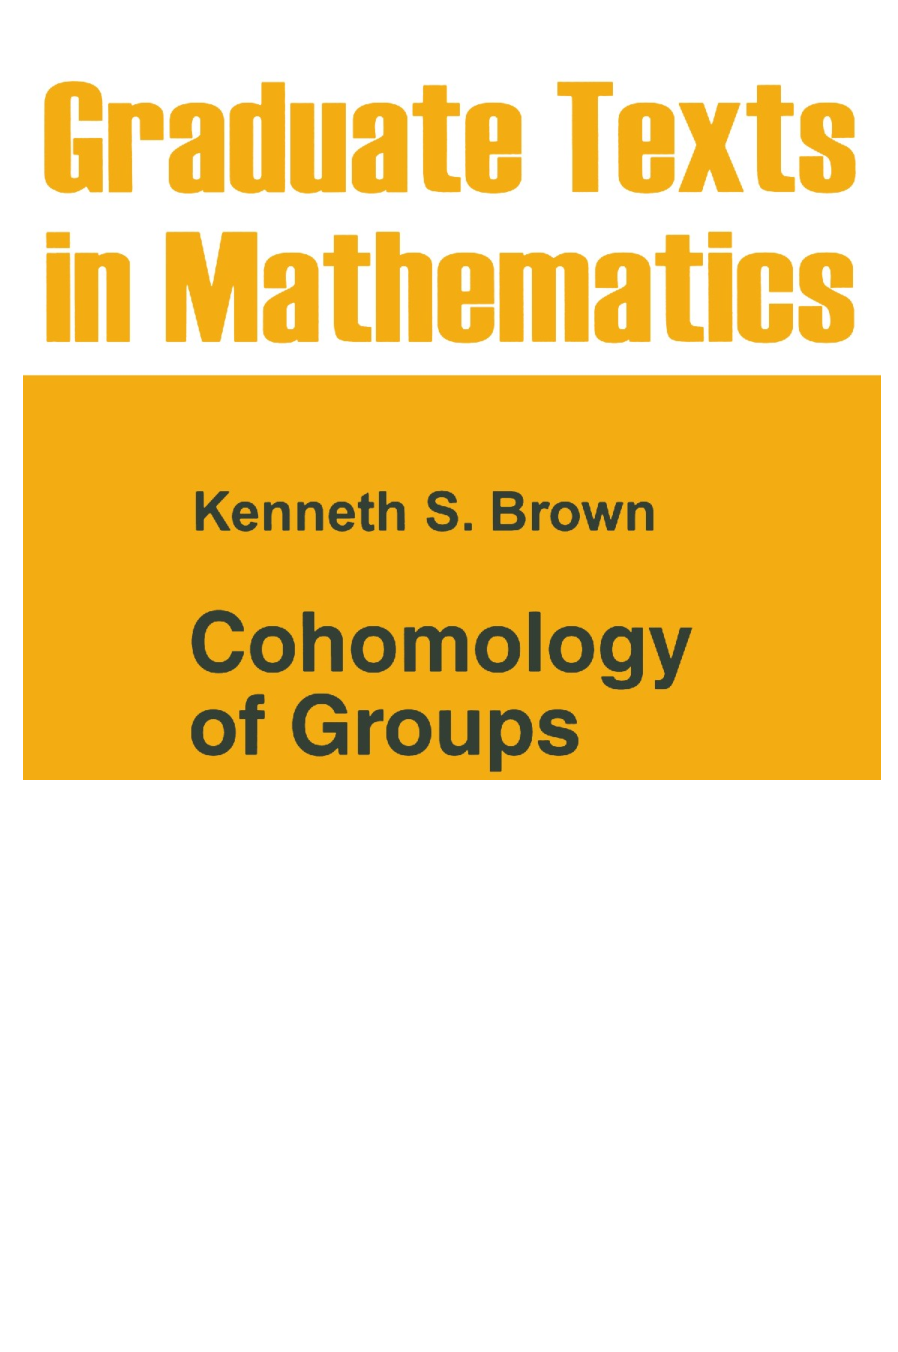
\includegraphics[height=2cm]{brown_book}
	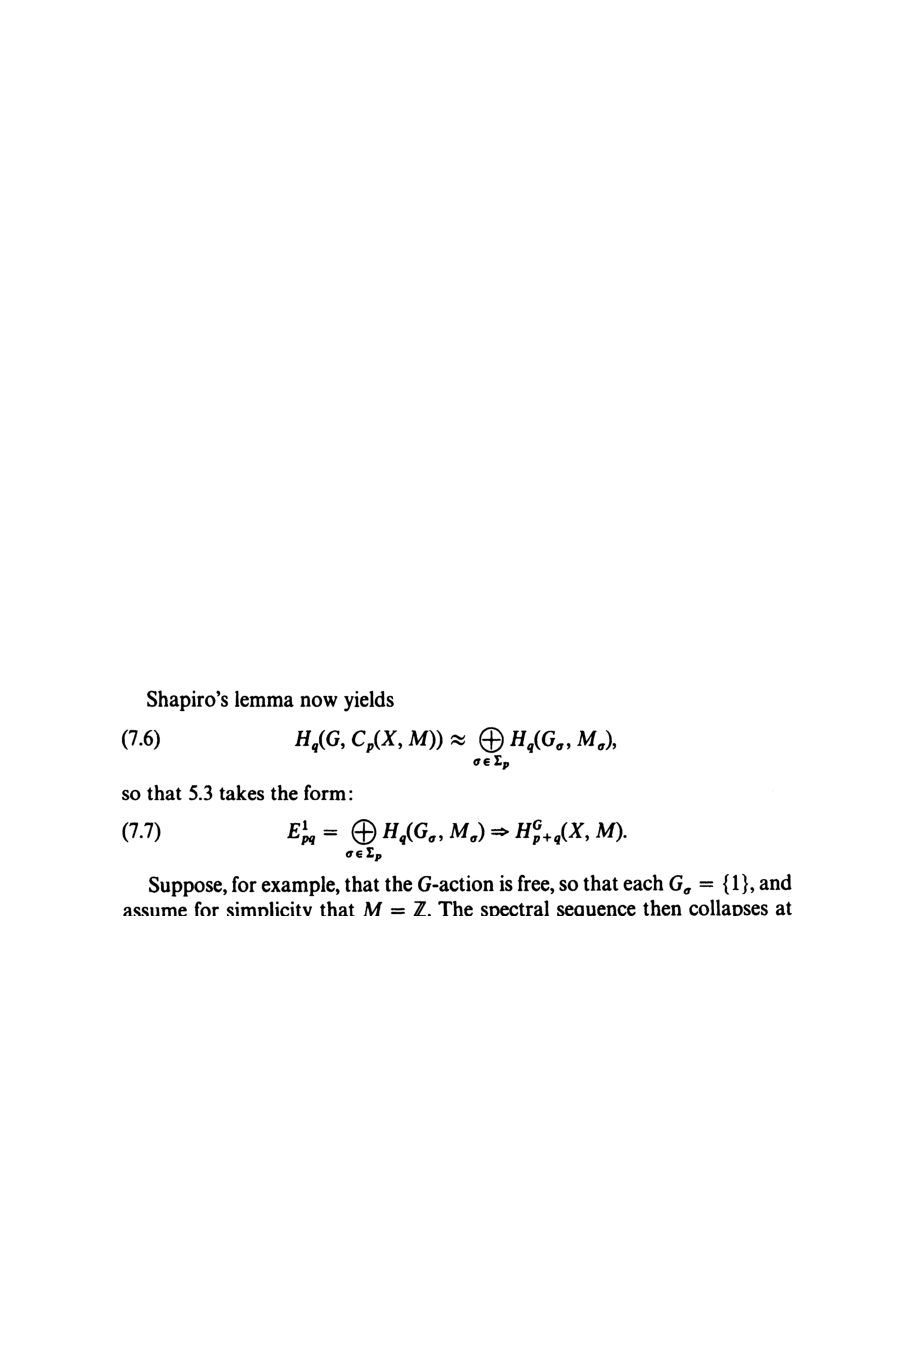
\includegraphics[height=2cm]{brown_ss}
\end{center}
{\small Z. Song, C. Fang and YQ, Nat. Commun. \textbf{11}, 4197 (2020).}
\end{frame}

\begin{frame}
  \frametitle{An example of a nontrivial building block}
  \begin{columns}
    \column{.7\textwidth}
    \begin{itemize}
      \item<1-> Consider $G=SG\times\mathbb Z_2$, $SG=P4_22_12$ (\#94 space group).
      \item<2-> Each colored 2-cell is decorated with a Levin-Gu or CZX state protected by the onsite $\mathbb Z_2$.
      \item<3-> Each edge borders two decorated 2-cells: edge states canceled out.
      \item<4-> Forms a nontrivial TCS.
    \end{itemize}
    \column{.3\textwidth}
    \includegraphics[height=4cm]{blocks}
    \end{columns}
  \end{frame}
  
  \begin{frame}
    \frametitle{Results for all 230 space groups}
    \begin{center}
      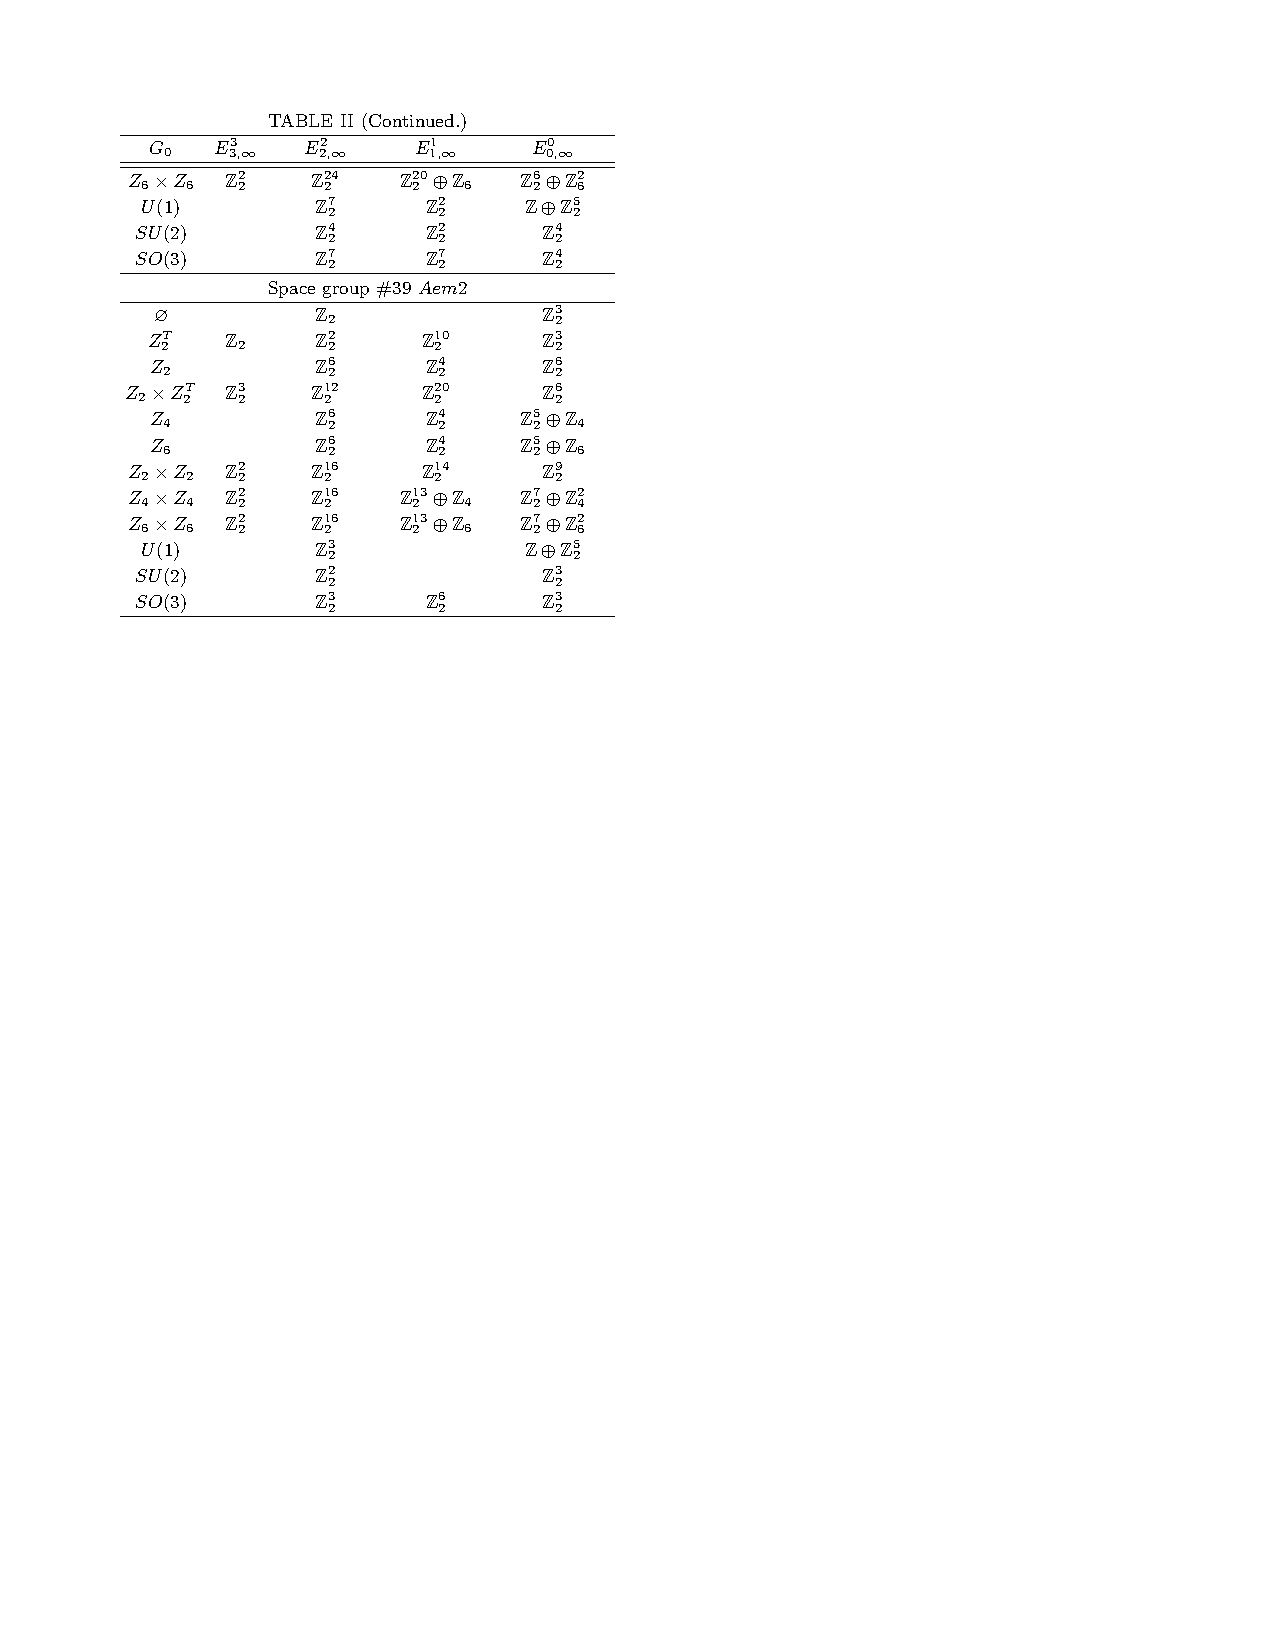
\includegraphics[height=8cm]{bigtable}
    \end{center}
  \end{frame}
  
  \begin{frame}
  \frametitle{An example of 2nd order computation}
  \emph{\small Adapted from Xu Yang, Shenghan Jiang, Ashvin Vishwanath and Ying Ran, Ann. Phys. 413, 168060 (2020).}
  \begin{itemize}
    \item Consider a magnetic translation symmetry $T_xT_yT_x^{-1}T_y^{-1} = X$, and $G_0=\mathbb Z_2^X\times\mathbb Z_2^T$.
    \item $H^3[G_0,\uone_T]=\mathbb Z_2\oplus\mathbb Z_2$: the one protected by both $\mathbb Z_2^X$ and $\mathbb Z_2^T$ is \alert{not compatible} with the magnetic translation symmetry.
    \item Try to decorate $\omega\in H^3[G_0,\uone_T]$ to all 2-cells: the 1-cells can be gapped out, but the 0-cells \alert{cannot}.
    \item There must be a $T^2=-1$ Kramers doublet at each 0-cell.
  \end{itemize}
  \begin{center}
  \begin{tikzpicture}
  \draw (-1.2,0)--(1.2,0);
  \draw (-1.2,1)--(1.2,1);
  \draw (-1.2,-1)--(1.2,-1);
  \draw (-1,-1.2)--(-1,1.2);
  \draw (0,-1.2)--(0,1.2);
  \draw (1,-1.2)--(1,1.2);
  \fill [red] (-1,-1) circle (2pt);
  \fill [red] (-1,0) circle (2pt);
  \fill [red] (-1,1) circle (2pt);
  \fill [red] (0,-1) circle (2pt);
  \fill [red] (0,0) circle (2pt);
  \fill [red] (0,1) circle (2pt);
  \fill [red] (1,-1) circle (2pt);
  \fill [red] (1,0) circle (2pt);
  \fill [red] (1,1) circle (2pt);
  \end{tikzpicture}
  \end{center}
  \end{frame}
  
\begin{frame}
  \frametitle{Real-space construction of fSPTs}

  \begin{itemize}
  \item Interacting fSPTs:
    \begin{itemize}
    \item 2D point groups: Jian-Hao Zhang, Qing-Rui Wang, Shuo Yang, YQ and Zheng-Cheng Gu,
      PRB \textbf{101}, 100501(R) (2020).
    \item 2D wallpaper groups: Jian-Hao Zhang, Shuo Yang, YQ and Zheng-Cheng Gu,
      PR Research \textbf{4}, 033081 (2022).
    \item 3D point groups: Jian-Hao Zhang, YQ and Zheng-Cheng Gu, arXiv:2204.13558.
    \end{itemize}
  \item Free-fermion high-order states:
    Tian Yuan, Chen Fang and YQ, to appear.
  \end{itemize}
  \begin{center}
    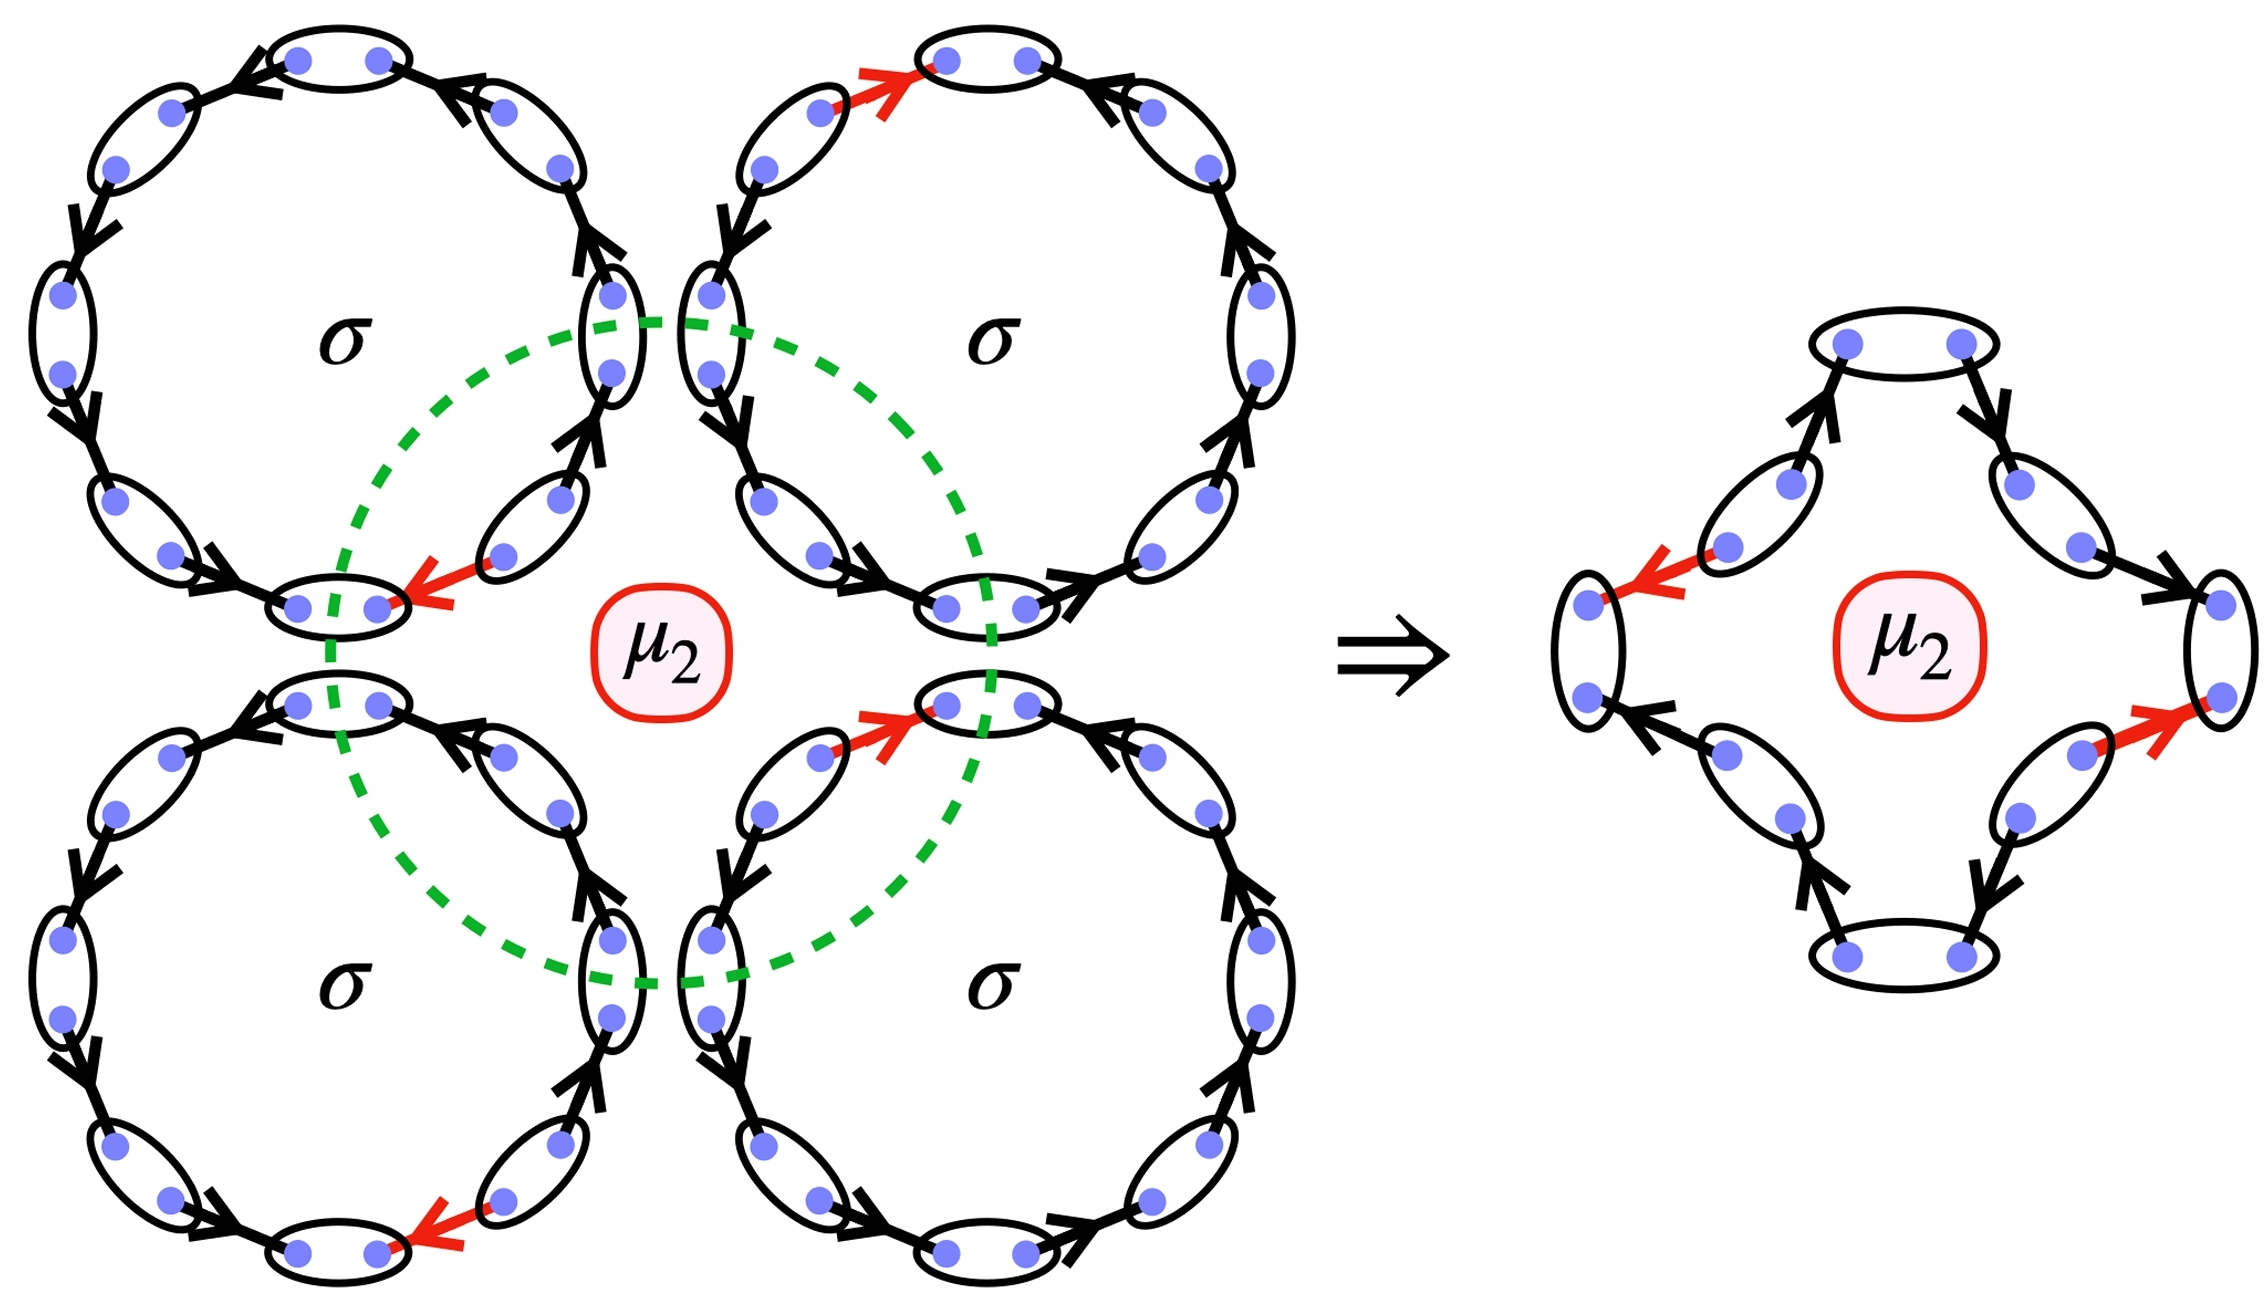
\includegraphics[height=4cm]{majorana_bubble}    
  \end{center}
\end{frame}

\section{Conclusion}

\begin{frame}
\frametitle{Summary: towards a complete classification of TCS}
\begin{itemize}
\item Crystalline symmetry: treat as onsite symmetry / real-space construction.
\item Treat as onsite symmetry:
  \begin{itemize}
  \item 1D \ding{51}, 2D \ding{51}, 3D ??
  \item SptSet package: work in progress.
  \end{itemize}
\item Real-space construction
  \begin{itemize}
  \item General rules are known.
  \item Many examples are studied.
  \item Automated computation for interacting-fermion systems?
  \end{itemize}
\item Crosschecked results using the crystalline equivalence principle.
\end{itemize}
\end{frame}

\end{document}
